\documentclass[11pt,a4paper]{article}

\usepackage{amsfonts,amssymb,amsmath}
\usepackage[margin=1in]{geometry}
\usepackage[none]{hyphenat}
\usepackage{graphicx}
\usepackage{fancyhdr}
\usepackage{float}
\usepackage{color}
\usepackage{xcolor}
\usepackage{tikz}
\usepackage[nottoc,notlot,notlof]{tocbibind}

\usetikzlibrary{arrows.meta,patterns,shapes}

\parindent 0ex
\setlength{\parskip}{0.55\baselineskip}
% Displays carry their own skips; with a non-zero \parskip on top of them,
% consecutive displays drift apart. Tighten them so a derivation reads as one
% argument rather than as a column of disconnected formulae.
\setlength{\abovedisplayskip}{0.5\baselineskip}
\setlength{\belowdisplayskip}{0.5\baselineskip}
\setlength{\abovedisplayshortskip}{0.25\baselineskip}
\setlength{\belowdisplayshortskip}{0.25\baselineskip}
% Equations numbered within sections, (2.1), (2.2), ..., to sit with the
% section.subsection.n numbering of the theorem environments below.
\numberwithin{equation}{section}

\pagestyle{fancy}
\fancyfoot[C]{\thepage}
\fancyhead{}
\fancyhead[R]{\rightmark}
\renewcommand{\headrulewidth}{0pt}

% Theorem environments.
\usepackage{amsthm}
\theoremstyle{definition}
% One shared counter running section.subsection.n, as in the other courses here.
\newtheorem{thm}{Theorem}[subsection]
\newtheorem{defn}[thm]{Definition}
\newtheorem{exa}[thm]{Example}
\newtheorem{prop}[thm]{Proposition}
\newtheorem{coro}[thm]{Corollary}
\newtheorem{lem}[thm]{Lemma}
\newtheorem{result}[thm]{Result}
\newtheorem{exe}[thm]{Exercise}
\newtheorem*{note}{Note}
\newtheorem*{remark}{Remark}
\newtheorem{problemx}{Problem}[subsection]
\newenvironment{problem}{\begin{problemx}}{\end{problemx}}
\newenvironment{solution}
  {\renewcommand{\qedsymbol}{}\begin{proof}[\textit{Solution}.]}
  {\end{proof}}
\usepackage{enumitem}
% A heading that is legal inside a theorem body, a list or a float, where
% \subsubsection is not. Same weight as \subsubsection* so the two read alike.
\newcommand{\subhead}[1]{%
  \par\medskip\noindent\textbf{#1}\par\nobreak\smallskip}

\begin{document}
% Title page depersonalised for the web, as with every other course here: no
% university, no lecturers, no author, no year. The identity kept below is the
% least-squares estimator, which the whole course builds towards and then tests.
\begin{titlepage}
\thispagestyle{empty}
\begin{center}
\vspace*{3cm}
{\Huge\bfseries Regression Analysis}\\[1.2cm]
{\large Lecture Notes}\\[2.5cm]
\line(1,0){300}\\[1.5cm]
$$\hat{\boldsymbol\beta} = (\mathbf{X}^\top \mathbf{X})^{-1} \mathbf{X}^\top \mathbf{y}$$
\end{center}
\end{titlepage}

\tableofcontents
\thispagestyle{empty}
\clearpage
\setcounter{page}{1}








\section{Introduction}
Regression Analysis is a statistical tool for investigating the relationship between a dependent variable and one or more independent variables.

Regression analysis is widely used for prediction and forecasting.


\begin{exa}\label{exa:disney}
You are a marketing analyst for Disney Toys. You gather the following data:
\begin{center}
\begin{tabular}{l|ccccc}
Ad (\$) & 1 & 2 & 3 & 4 & 5 \\
\hline
Sales (units) & 1 & 1 & 2 & 2 & 4 \\
\end{tabular}
\end{center}
We let
\begin{itemize}
\item advertising $X$ be the regressor variable (independent);
\item sales $Y$ be the response variable (dependent).
\end{itemize}
What is the relationship between sales and advertising?
\end{exa}

\begin{note}
We can control the advertising $X$; the sales $Y$ we can only observe.
\end{note}


\subsection{Scatter plot}
A scatter plot is a diagram that displays the values of two variables for a set of data,
one point $(X_i, Y_i)$ for each observation. For the advertising data of
Example~\ref{exa:disney}:

% The data columns are drawn inside the picture rather than set as a tabular in
% a second minipage: on the web, minipages stack, and the table landed under
% the diagram instead of beside it.
\begin{figure}[H]
\centering
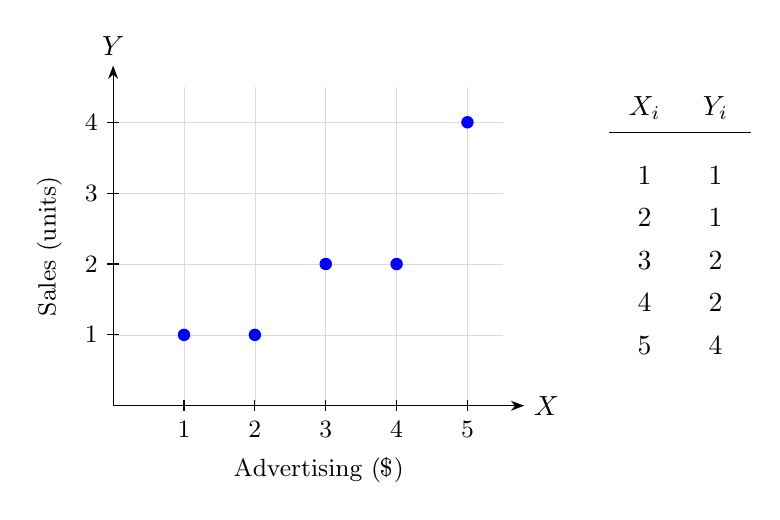
\begin{tikzpicture}[scale=0.9]
\draw[step=1,gray!30,very thin] (0,0) grid (5.5,4.5);
\draw[-Stealth] (0,0) -- (5.8,0) node[right] {$X$};
\draw[-Stealth] (0,0) -- (0,4.8) node[above] {$Y$};
\foreach \x in {1,...,5} \draw (\x,0.08) -- (\x,-0.08) node[below] {\small $\x$};
\foreach \y in {1,...,4} \draw (0.08,\y) -- (-0.08,\y) node[left] {\small $\y$};
\foreach \p in {(1,1),(2,1),(3,2),(4,2),(5,4)} \fill[blue] \p circle (2.5pt);
\node[below] at (2.9,-0.6) {\small Advertising (\$)};
\node[rotate=90] at (-0.9,2.25) {\small Sales (units)};
% The data, in columns to the right of the axes.
\node at (7.5,4.2) {$X_i$};
\node at (8.5,4.2) {$Y_i$};
\draw (7,3.85) -- (9,3.85);
\foreach \x/\y [count=\r] in {1/1,2/1,3/2,4/2,5/4} {
  \node at (7.5,3.85-0.6*\r) {$\x$};
  \node at (8.5,3.85-0.6*\r) {$\y$};
}
\end{tikzpicture}
\caption{Scatter plot of sales against advertising.}
\end{figure}

Scatter plots are used to investigate the possible relationship between the variables.
Here the points rise from left to right, roughly along a straight line: more advertising
goes with more sales.

A scatter plot should always be drawn before any model is fitted. It shows at a glance
whether a straight line is sensible at all, and points that do not fit the pattern.

\subsection{Statistical and deterministic relationships}
A relationship such as $F = \frac95 C + 32$ between temperatures in Fahrenheit and Celsius is
\textbf{deterministic}: given $C$, the value of $F$ is fixed exactly. The relationship between
advertising and sales is not like that. Two weeks with the same advertising spend will not
give the same sales, because sales depend on many other things we have not measured. Such a
relationship is \textbf{statistical}: $x$ determines the \emph{average} value of $y$, and
individual values scatter about that average. A regression model has two parts accordingly,
\[
\text{response} = \underbrace{\text{systematic part}}_{\text{depends on } x}
               + \underbrace{\text{random error}}_{\text{everything else}} .
\]

\subsection{What ``linear'' means}
A regression model is called \textbf{linear} when it is linear in the \emph{parameters}
$\beta_0, \beta_1, \dots$, not necessarily in $x$. For example,
\begin{align*}
y &= \beta_0 + \beta_1 x + \varepsilon && \text{(a straight line: linear)}, \\
y &= \beta_0 + \beta_1 x + \beta_2 x^2 + \varepsilon && \text{(a parabola: still linear)}, \\
y &= \beta_0 + \beta_1 \log x + \varepsilon && \text{(linear)}, \\
y &= \beta_0 e^{\beta_1 x} + \varepsilon && \text{(nonlinear in $\beta_1$)} .
\end{align*}
In the first three, each parameter multiplies a known quantity and the terms are added, so
the same estimation method works for all of them. The last is a \textbf{nonlinear}
regression model, treated in a later section.

A model with one regressor is a \textbf{simple} regression model; with two or more it is a
\textbf{multiple} regression model.

\subsection{Uses of regression}
\begin{enumerate}
\item \textbf{Description.} Summarising how $y$ changes with $x$, for example by how much mean
sales rise for each extra dollar of advertising.
\item \textbf{Prediction and forecasting.} Estimating $y$ for a value of $x$ that has not been
observed, within the range of the data.
\item \textbf{Control.} Choosing $x$ to give a desired value of $y$, for example the
advertising spend needed for a sales target.
\item \textbf{Estimation of parameters} that have a scientific meaning, such as a rate of
reaction.
\end{enumerate}

\begin{remark}
Regression establishes association, not causation. A strong relationship between $x$ and $y$
in observational data may be due to a third variable that drives both. Only a designed
experiment, in which $x$ is set by the investigator, supports a causal conclusion.
\end{remark}

The name has a history. Francis Galton, studying the heights of parents and their children
in the 1880s, found that children of unusually tall parents were on average shorter than
their parents, and children of unusually short parents taller: their heights
``regressed'' towards the mean. The method he used to describe this kept the name.

\subsection{Steps in a regression analysis}
\begin{enumerate}
\item State the problem and choose the response and the regressors.
\item Collect the data, by a designed experiment where possible.
\item Plot the data.
\item Specify a model, and fit it: estimate the parameters.
\item Check the model: are the assumptions reasonable, and does it fit
(Model adequacy checking, Test for influential observations)?
\item If it is inadequate, revise it and fit again (Transformation \& weighting, and the
sections that follow).
\item Use the model, for description, prediction or control.
\end{enumerate}













\section{Simple linear regression}
A simple linear regression model is a model with a single regressor $X$ that has a linear relationship with a response $Y$. The simple linear regression model is 
\begin{equation}
Y = \beta_0 + \beta_1X + \varepsilon
\end{equation}
where
\begin{itemize}
\item $Y$ is the response variable;
\item $X$ is the regressor variable;
\item $\beta_0$ is the intercept;
\item $\beta_1$ is the slope;
\item $\varepsilon$ is the random error component.
\end{itemize}

\begin{note}
$Y$ is a random variable, because $\varepsilon$ is.
\end{note}

\begin{remark}
For a given $X$, the corresponding observation $Y$ consists of the value $\, \beta_0 + \beta_1X\,$ plus an amount $\varepsilon$.
\end{remark}

\subsection{The model and its assumptions}
Suppose we have $n$ pairs of observations $(x_1,y_1), (x_2,y_2), \dots, (x_n,y_n)$. From
here on we follow the usual convention and write the sample values in lower case: the
$x_i$ are treated as fixed, known constants (we chose them, or we condition on them), and
each $y_i$ is the value taken by a random variable. The model for the sample is
\begin{equation}\label{eq:slr-sample}
y_i = \beta_0 + \beta_1 x_i + \varepsilon_i, \qquad i = 1, 2, \dots, n.
\end{equation}

We now make some basic assumptions on the errors $\varepsilon_i$:
\begin{enumerate}[label=\textbf{A\arabic*.}]
\item $E(\varepsilon_i) = 0$ for every $i$: the errors average out to zero;
\item $\operatorname{Var}(\varepsilon_i) = \sigma^2$ for every $i$: the spread is the same at every $x$ (\emph{constant variance}, or \emph{homoscedasticity});
\item $\operatorname{Cov}(\varepsilon_i, \varepsilon_j) = 0$ for $i \neq j$: the errors are \emph{uncorrelated};
\item $\varepsilon_i \sim N(0, \sigma^2)$: the errors are normally distributed.
\end{enumerate}
Assumptions A1--A3 are all that least-squares estimation needs, and the results of the
next four subsections rest on them alone. The normality assumption A4 is needed for tests
and confidence intervals, from Subsection~\ref{ssec:distributions} on. Together, A3 and A4
make the errors independent, since uncorrelated normal variables are independent.

\begin{thm}\label{thm:mean-var-y}
Under A1--A3, for each $i$,
\[
E(y_i) = \beta_0 + \beta_1 x_i, \qquad \operatorname{Var}(y_i) = \sigma^2, \qquad
\operatorname{Cov}(y_i, y_j) = 0 \quad (i \neq j).
\]
\end{thm}

\begin{proof}
Since $\beta_0 + \beta_1 x_i$ is a constant,
$E(y_i) = \beta_0 + \beta_1 x_i + E(\varepsilon_i) = \beta_0 + \beta_1 x_i$ by A1. Adding a
constant does not change a variance or a covariance, so
$\operatorname{Var}(y_i) = \operatorname{Var}(\varepsilon_i) = \sigma^2$ by A2 and
$\operatorname{Cov}(y_i,y_j) = \operatorname{Cov}(\varepsilon_i,\varepsilon_j) = 0$ by A3.
\end{proof}

So the line $\beta_0 + \beta_1 x$ is the line of \emph{means}: at each value of $x$, the
response is scattered about the point on the line, with the same spread $\sigma$ everywhere.
With A4 the scatter is normal, as in Figure~\ref{fig:slr-assumptions}.

\begin{figure}[H]
\centering
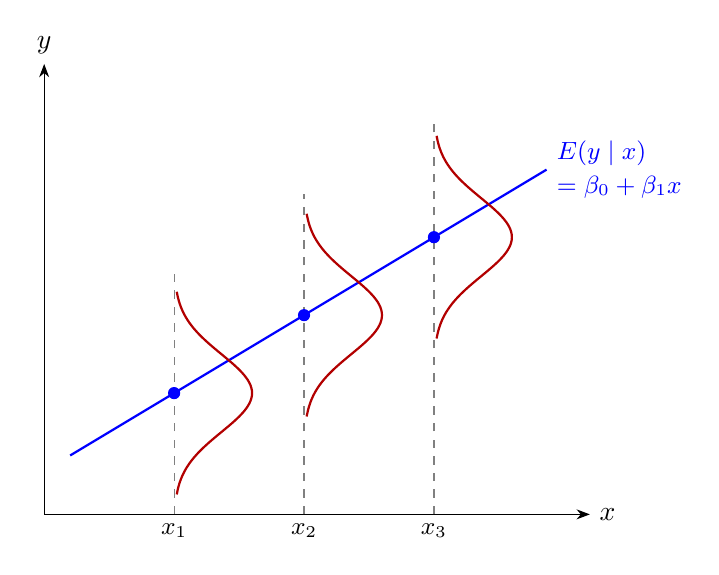
\begin{tikzpicture}[scale=1.1]
\draw[-Stealth] (0,0) -- (6.3,0) node[right] {$x$};
\draw[-Stealth] (0,0) -- (0,5.2) node[above] {$y$};
\draw[thick,blue] (0.3,0.68) -- (5.8,3.98)
  node[right,align=left] {\small $E(y \mid x)$\\ \small $=\beta_0+\beta_1 x$};
\foreach \xo [count=\k] in {1.5,3,4.5} {
  \draw[dashed,gray] (\xo,0) -- (\xo,{0.5+0.6*\xo+1.4});
  \draw[thick,red!70!black] plot[domain=-2.6:2.6,samples=40,smooth]
    ({\xo+0.9*exp(-0.5*(\x)^2)},{0.5+0.6*\xo+0.45*\x});
  \fill[blue] (\xo,{0.5+0.6*\xo}) circle (2pt);
  \node[below] at (\xo,0) {\small $x_{\k}$};
}
\end{tikzpicture}
\caption{The simple linear regression model. At each $x$ the response is normal, centred
on the line, with the same variance $\sigma^2$.}
\label{fig:slr-assumptions}
\end{figure}

\subsection{Least-squares estimation of the parameters}
The parameters $\beta_0$ and $\beta_1$ are unknown and must be estimated from the data. The
method of \textbf{least squares} chooses the line that makes the sum of the squared
vertical distances from the points to the line as small as possible.

\begin{defn}
The \textbf{least-squares criterion} is
\[
S(\beta_0, \beta_1) = \sum_{i=1}^n \left( y_i - \beta_0 - \beta_1 x_i \right)^2 .
\]
The \textbf{least-squares estimators} $\hat\beta_0, \hat\beta_1$ are the values of
$\beta_0, \beta_1$ that minimise $S$.
\end{defn}

Before solving, we fix some notation that will be used throughout the course.

\begin{defn}
With $\bar x = \frac1n\sum x_i$ and $\bar y = \frac1n\sum y_i$,
\begin{align*}
S_{xx} &= \sum_{i=1}^n (x_i - \bar x)^2, \\
S_{xy} &= \sum_{i=1}^n (x_i - \bar x)(y_i - \bar y), \\
S_{yy} &= \sum_{i=1}^n (y_i - \bar y)^2 .
\end{align*}
\end{defn}

\begin{lem}\label{lem:sxx}
\begin{enumerate}[label=(\roman*)]
\item $\sum_{i=1}^n (x_i - \bar x) = 0$;
\item $S_{xx} = \sum x_i^2 - n\bar x^2 = \sum x_i^2 - \dfrac{\left(\sum x_i\right)^2}{n}$;
\item $S_{xy} = \sum (x_i - \bar x) y_i = \sum x_i y_i - n \bar x \bar y
       = \sum x_i y_i - \dfrac{\left(\sum x_i\right)\left(\sum y_i\right)}{n}$.
\end{enumerate}
The same holds for $S_{yy}$ with $y$ in place of $x$.
\end{lem}

\begin{proof}
(i) $\sum (x_i - \bar x) = \sum x_i - n\bar x = n\bar x - n\bar x = 0$.

(ii) Expanding the square,
\begin{align*}
S_{xx} &= \sum \left(x_i^2 - 2\bar x x_i + \bar x^2\right)
        = \sum x_i^2 - 2\bar x \sum x_i + n\bar x^2 \\
       &= \sum x_i^2 - 2n\bar x^2 + n\bar x^2
        = \sum x_i^2 - n\bar x^2 ,
\end{align*}
and $n\bar x^2 = n\left(\sum x_i / n\right)^2 = \left(\sum x_i\right)^2/n$.

(iii) $S_{xy} = \sum (x_i - \bar x) y_i - \bar y \sum (x_i - \bar x) = \sum (x_i - \bar x) y_i$
by (i). Then
$\sum (x_i - \bar x) y_i = \sum x_i y_i - \bar x \sum y_i = \sum x_i y_i - n\bar x \bar y$.
\end{proof}

The forms with $\sum x_i^2$ and $\sum x_i y_i$ are the ones to use by hand: they need only
the column totals of a table, as in the examples below.

\begin{thm}[Least-squares estimators]\label{thm:ls}
Provided the $x_i$ are not all equal, the least-squares estimators of $\beta_1$ and $\beta_0$
are
\[
\boxed{\;\hat\beta_1 = \frac{S_{xy}}{S_{xx}}, \qquad \hat\beta_0 = \bar y - \hat\beta_1 \bar x\;}
\]
and the \textbf{fitted regression line} is $\hat y = \hat\beta_0 + \hat\beta_1 x$.
\end{thm}

\begin{proof}
At a minimum of $S$ both partial derivatives vanish:
\begin{align*}
\frac{\partial S}{\partial \beta_0} &= -2 \sum \left( y_i - \beta_0 - \beta_1 x_i \right) = 0, \\
\frac{\partial S}{\partial \beta_1} &= -2 \sum x_i \left( y_i - \beta_0 - \beta_1 x_i \right) = 0 .
\end{align*}
Dividing by $-2$ and rearranging gives the \textbf{normal equations}
% Unnumbered, and referred to in words: tex4ht cannot resolve a \label inside
% align on the web, where an \eqref to one prints as (??).
\begin{align*}
n\hat\beta_0 + \hat\beta_1 \sum x_i &= \sum y_i, \\
\hat\beta_0 \sum x_i + \hat\beta_1 \sum x_i^2 &= \sum x_i y_i .
\end{align*}
Dividing the first normal equation by $n$ gives $\hat\beta_0 + \hat\beta_1 \bar x = \bar y$,
that is, $\hat\beta_0 = \bar y - \hat\beta_1 \bar x$. Substituting this into the second,
\[
(\bar y - \hat\beta_1 \bar x)\, n\bar x + \hat\beta_1 \sum x_i^2 = \sum x_i y_i ,
\]
and collecting the terms in $\hat\beta_1$,
\[
\hat\beta_1 \left( \sum x_i^2 - n\bar x^2 \right) = \sum x_i y_i - n\bar x\bar y ,
\]
which by Lemma~\ref{lem:sxx} reads $\hat\beta_1 S_{xx} = S_{xy}$. Since the $x_i$ are not all
equal, $S_{xx} > 0$ and we may divide.

It remains to check that this stationary point is a minimum. The second derivatives are
\[
\frac{\partial^2 S}{\partial \beta_0^2} = 2n, \qquad
\frac{\partial^2 S}{\partial \beta_1^2} = 2\sum x_i^2, \qquad
\frac{\partial^2 S}{\partial \beta_0 \, \partial \beta_1} = 2\sum x_i ,
\]
constants, so the Hessian matrix is the same at every point. Its leading entry $2n$ is
positive and its determinant is
\[
4n\sum x_i^2 - 4\left(\sum x_i\right)^2 = 4n\left( \sum x_i^2 - n\bar x^2 \right) = 4nS_{xx} > 0 .
\]
The Hessian is therefore positive definite everywhere, $S$ is a convex function, and the
stationary point is its global minimum.
\end{proof}

\begin{note}
If all the $x_i$ are equal then $S_{xx} = 0$ and the slope cannot be estimated: every line
through the point $(x_1, \bar y)$ fits equally well. To learn how $y$ changes with $x$, the
data must contain different values of $x$.
\end{note}

\begin{defn}
The \textbf{fitted value} at $x_i$ is $\hat y_i = \hat\beta_0 + \hat\beta_1 x_i$, and the
\textbf{residual} is $e_i = y_i - \hat y_i$, the vertical distance from the $i$th point to
the fitted line.
\end{defn}

The residual $e_i$ is observed; the error $\varepsilon_i = y_i - \beta_0 - \beta_1 x_i$ is
not, because $\beta_0$ and $\beta_1$ are unknown. The residuals are our estimates of the
errors.

\begin{exa}\label{exa:disney-fit}
Fit the least-squares line to the advertising data of Example~\ref{exa:disney}, and interpret
the estimates.
\end{exa}

\begin{solution}
Set out the working in a table, one row per observation, and add up the columns:
\begin{center}
\begin{tabular}{c|ccccc}
$i$ & $x_i$ & $y_i$ & $x_i^2$ & $x_i y_i$ & $y_i^2$ \\
\hline
1 & 1 & 1 & 1 & 1 & 1 \\
2 & 2 & 1 & 4 & 2 & 1 \\
3 & 3 & 2 & 9 & 6 & 4 \\
4 & 4 & 2 & 16 & 8 & 4 \\
5 & 5 & 4 & 25 & 20 & 16 \\
\hline
$\sum$ & 15 & 10 & 55 & 37 & 26 \\
\end{tabular}
\end{center}
So $n = 5$, $\bar x = 15/5 = 3$ and $\bar y = 10/5 = 2$. By Lemma~\ref{lem:sxx},
\begin{align*}
S_{xx} &= 55 - \frac{15^2}{5} = 55 - 45 = 10, \\
S_{xy} &= 37 - \frac{15 \times 10}{5} = 37 - 30 = 7 .
\end{align*}
By Theorem~\ref{thm:ls},
\[
\hat\beta_1 = \frac{S_{xy}}{S_{xx}} = \frac{7}{10} = 0.7, \qquad
\hat\beta_0 = \bar y - \hat\beta_1 \bar x = 2 - 0.7 \times 3 = -0.1 ,
\]
and the fitted line is
\[
\hat y = -0.1 + 0.7x .
\]
\textbf{Interpretation.} The slope says that each extra dollar of advertising goes with an
increase of $0.7$ units in \emph{mean} sales. The intercept would be the mean sales with no
advertising at all, but $x = 0$ lies outside the data, which run from $1$ to $5$, and
negative sales are impossible. The intercept here is simply where the line has to cross the
axis to fit the observed range; it should not be read as a prediction. Using a fitted line
outside the range of the data is called \textbf{extrapolation}, and it is unreliable.

The fitted values and residuals are
\begin{center}
\begin{tabular}{c|ccccc}
$x_i$ & 1 & 2 & 3 & 4 & 5 \\
\hline
$y_i$ & 1 & 1 & 2 & 2 & 4 \\
$\hat y_i = -0.1 + 0.7x_i$ & 0.6 & 1.3 & 2.0 & 2.7 & 3.4 \\
$e_i = y_i - \hat y_i$ & 0.4 & $-0.3$ & 0.0 & $-0.7$ & 0.6 \\
\end{tabular}
\end{center}
They are shown as the vertical segments in Figure~\ref{fig:disney-fit}.
\end{solution}

\begin{figure}[H]
\centering
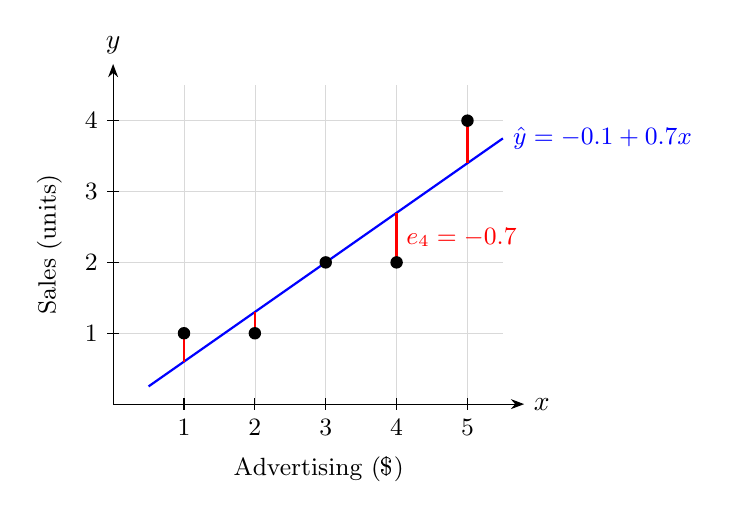
\begin{tikzpicture}[scale=0.9]
\draw[step=1,gray!30,very thin] (0,0) grid (5.5,4.5);
\draw[-Stealth] (0,0) -- (5.8,0) node[right] {$x$};
\draw[-Stealth] (0,0) -- (0,4.8) node[above] {$y$};
\foreach \x in {1,...,5} \draw (\x,0.08) -- (\x,-0.08) node[below] {\small $\x$};
\foreach \y in {1,...,4} \draw (0.08,\y) -- (-0.08,\y) node[left] {\small $\y$};
\draw[thick,blue] (0.5,0.25) -- (5.5,3.75) node[right] {\small $\hat y = -0.1 + 0.7x$};
\foreach \x/\y in {1/1,2/1,3/2,4/2,5/4} {
  \draw[red,thick] (\x,\y) -- (\x,{-0.1+0.7*\x});
  \fill[black] (\x,\y) circle (2.5pt);
}
\node[red,right] at (4,2.35) {\small $e_4 = -0.7$};
\node[below] at (2.9,-0.6) {\small Advertising (\$)};
\node[rotate=90] at (-0.9,2.25) {\small Sales (units)};
\end{tikzpicture}
\caption{The least-squares line for the advertising data. The red segments are the
residuals; least squares makes the sum of their squares as small as possible.}
\label{fig:disney-fit}
\end{figure}

\begin{exa}\label{exa:yield}
In a chemical process, the yield $y$ (\%) was recorded at six temperatures $x$ ($^\circ$C):
\begin{center}
\begin{tabular}{l|cccccc}
Temperature $x$ & 10 & 20 & 30 & 40 & 50 & 60 \\
\hline
Yield $y$ & 52 & 58 & 63 & 70 & 74 & 81 \\
\end{tabular}
\end{center}
Fit a straight line, and estimate the mean yield at $45^\circ$C.
\end{exa}

\begin{solution}
\begin{center}
\begin{tabular}{c|ccccc}
$i$ & $x_i$ & $y_i$ & $x_i^2$ & $x_i y_i$ & $y_i^2$ \\
\hline
1 & 10 & 52 & 100 & 520 & 2704 \\
2 & 20 & 58 & 400 & 1160 & 3364 \\
3 & 30 & 63 & 900 & 1890 & 3969 \\
4 & 40 & 70 & 1600 & 2800 & 4900 \\
5 & 50 & 74 & 2500 & 3700 & 5476 \\
6 & 60 & 81 & 3600 & 4860 & 6561 \\
\hline
$\sum$ & 210 & 398 & 9100 & 14930 & 26974 \\
\end{tabular}
\end{center}
Here $n = 6$, $\bar x = 210/6 = 35$ and $\bar y = 398/6 = 66.3333$. Then
\begin{align*}
S_{xx} &= 9100 - \frac{210^2}{6} = 9100 - 7350 = 1750, \\
S_{xy} &= 14930 - \frac{210 \times 398}{6} = 14930 - 13930 = 1000,
\end{align*}
so
\[
\hat\beta_1 = \frac{1000}{1750} = 0.5714, \qquad
\hat\beta_0 = 66.3333 - 0.5714 \times 35 = 46.3333 ,
\]
and the fitted line is $\hat y = 46.3333 + 0.5714x$. Each extra degree raises the mean
yield by about $0.57$ percentage points.

At $x = 45$, inside the range of the data,
$\hat y = 46.3333 + 0.5714 \times 45 = 72.05\%$.
\end{solution}

\begin{remark}
Carry plenty of decimal places in intermediate steps, or keep exact fractions. Here
$\hat\beta_1 = 4/7$ exactly; rounding it to $0.57$ before computing $\hat\beta_0$ would give
$\hat\beta_0 = 66.3333 - 0.57 \times 35 = 46.38$, already wrong in the second decimal place.
\end{remark}

\subsection{Properties of the fitted line}
The normal equations force the residuals to satisfy some exact identities. These are useful
for checking hand calculations, and they are used repeatedly in the proofs that follow.

\begin{thm}\label{thm:resid-props}
For the least-squares fit of a model with an intercept:
\begin{enumerate}[label=(\roman*)]
\item $\sum e_i = 0$: the residuals sum to zero;
\item $\sum y_i = \sum \hat y_i$;
\item $\sum x_i e_i = 0$;
\item $\sum \hat y_i e_i = 0$;
\item the fitted line passes through the point $(\bar x, \bar y)$.
\end{enumerate}
\end{thm}

\begin{proof}
The normal equations of Theorem~\ref{thm:ls} are $\sum (y_i - \hat\beta_0 - \hat\beta_1 x_i) = 0$
and $\sum x_i (y_i - \hat\beta_0 - \hat\beta_1 x_i) = 0$, and the bracket in each is exactly
$e_i$.

(i) and (iii) are therefore the two normal equations themselves.

(ii) By (i), $0 = \sum (y_i - \hat y_i) = \sum y_i - \sum \hat y_i$.

(iv) $\sum \hat y_i e_i = \sum (\hat\beta_0 + \hat\beta_1 x_i) e_i
= \hat\beta_0 \sum e_i + \hat\beta_1 \sum x_i e_i = 0$ by (i) and (iii).

(v) At $x = \bar x$ the line gives $\hat\beta_0 + \hat\beta_1 \bar x
= (\bar y - \hat\beta_1 \bar x) + \hat\beta_1 \bar x = \bar y$.
\end{proof}

\begin{exa}
Check (i) and (iii) for the residuals of Example~\ref{exa:disney-fit}.
\end{exa}

\begin{solution}
$\sum e_i = 0.4 - 0.3 + 0 - 0.7 + 0.6 = 0$, and
\begin{align*}
\sum x_i e_i &= 1(0.4) + 2(-0.3) + 3(0) + 4(-0.7) + 5(0.6) \\
             &= 0.4 - 0.6 + 0 - 2.8 + 3.0 = 0 .
\end{align*}
Both hold. Had either failed, there would be an arithmetic error in $\hat\beta_0$ or
$\hat\beta_1$.
\end{solution}

\begin{note}
(i) and (ii) depend on the model having an intercept: they come from the normal equation
for $\beta_0$. For a line forced through the origin they fail in general
(Problem~\ref{prob:origin}).
\end{note}

\subsection{Properties of the least-squares estimators}
The estimates $\hat\beta_0$ and $\hat\beta_1$ depend on the $y_i$, which are random; a new
sample at the same $x_i$ would give different estimates. So $\hat\beta_0$ and $\hat\beta_1$
are random variables, and we ask for their means and variances. Throughout, A1--A3 hold.

\begin{lem}\label{lem:ci}
$\hat\beta_1$ is a linear combination of the $y_i$:
\[
\hat\beta_1 = \sum_{i=1}^n c_i y_i, \qquad\text{where } c_i = \frac{x_i - \bar x}{S_{xx}} ,
\]
and the constants $c_i$ satisfy
\[
\sum c_i = 0, \qquad \sum c_i x_i = 1, \qquad \sum c_i^2 = \frac{1}{S_{xx}} .
\]
\end{lem}

\begin{proof}
By Lemma~\ref{lem:sxx}(iii), $\hat\beta_1 = S_{xy}/S_{xx} = \sum (x_i - \bar x) y_i / S_{xx} = \sum c_i y_i$.
Next, $\sum c_i = \sum (x_i - \bar x)/S_{xx} = 0$ by Lemma~\ref{lem:sxx}(i). For the second,
\[
\sum c_i x_i = \frac{\sum (x_i - \bar x) x_i}{S_{xx}} = \frac{S_{xx}}{S_{xx}} = 1 ,
\]
using Lemma~\ref{lem:sxx}(iii) with $y$ replaced by $x$, which says
$\sum (x_i - \bar x) x_i = S_{xx}$. Finally
$\sum c_i^2 = \sum (x_i - \bar x)^2 / S_{xx}^2 = S_{xx}/S_{xx}^2 = 1/S_{xx}$.
\end{proof}

\begin{thm}\label{thm:b1}
$\hat\beta_1$ is an unbiased estimator of $\beta_1$, with variance
\[
E(\hat\beta_1) = \beta_1, \qquad \operatorname{Var}(\hat\beta_1) = \frac{\sigma^2}{S_{xx}} .
\]
\end{thm}

\begin{proof}
By Lemma~\ref{lem:ci} and Theorem~\ref{thm:mean-var-y},
\begin{align*}
E(\hat\beta_1) &= \sum c_i E(y_i) = \sum c_i (\beta_0 + \beta_1 x_i) \\
  &= \beta_0 \sum c_i + \beta_1 \sum c_i x_i = \beta_0 \cdot 0 + \beta_1 \cdot 1 = \beta_1 .
\end{align*}
The $y_i$ are uncorrelated with common variance $\sigma^2$, so the variance of a linear
combination is the sum of the squared coefficients times $\sigma^2$:
\[
\operatorname{Var}(\hat\beta_1) = \sum c_i^2 \operatorname{Var}(y_i) = \sigma^2 \sum c_i^2 = \frac{\sigma^2}{S_{xx}} . \qedhere
\]
\end{proof}

\begin{remark}
$\operatorname{Var}(\hat\beta_1)$ is small when $S_{xx}$ is large, that is, when the $x_i$
are spread widely. When we can choose the $x$ values, as with advertising spend, spreading
them out gives a more precise slope.
\end{remark}

\begin{lem}\label{lem:cov-ybar}
$\operatorname{Cov}(\bar y, \hat\beta_1) = 0$.
\end{lem}

\begin{proof}
$\bar y = \sum \frac1n y_i$ and $\hat\beta_1 = \sum c_i y_i$. As the $y_i$ are uncorrelated
with variance $\sigma^2$,
\[
\operatorname{Cov}\Bigl(\sum \tfrac1n y_i, \sum c_j y_j\Bigr)
= \sum_i \tfrac1n c_i \operatorname{Var}(y_i) = \frac{\sigma^2}{n} \sum c_i = 0 . \qedhere
\]
\end{proof}

\begin{thm}\label{thm:b0}
$\hat\beta_0$ is an unbiased estimator of $\beta_0$, and
\[
\operatorname{Var}(\hat\beta_0) = \sigma^2 \left( \frac1n + \frac{\bar x^2}{S_{xx}} \right),
\qquad
\operatorname{Cov}(\hat\beta_0, \hat\beta_1) = -\frac{\bar x \sigma^2}{S_{xx}} .
\]
\end{thm}

\begin{proof}
$E(\bar y) = \frac1n \sum (\beta_0 + \beta_1 x_i) = \beta_0 + \beta_1 \bar x$, so by
Theorem~\ref{thm:b1}
\[
E(\hat\beta_0) = E(\bar y) - \bar x E(\hat\beta_1) = \beta_0 + \beta_1 \bar x - \bar x \beta_1 = \beta_0 .
\]
For the variance, $\operatorname{Var}(\bar y) = \sigma^2/n$, and by Lemma~\ref{lem:cov-ybar}
the covariance term vanishes:
\[
\operatorname{Var}(\hat\beta_0) = \operatorname{Var}(\bar y) + \bar x^2 \operatorname{Var}(\hat\beta_1)
- 2\bar x \operatorname{Cov}(\bar y, \hat\beta_1)
= \frac{\sigma^2}{n} + \frac{\bar x^2 \sigma^2}{S_{xx}} .
\]
Finally, again using Lemma~\ref{lem:cov-ybar},
\begin{align*}
\operatorname{Cov}(\hat\beta_0, \hat\beta_1) &= \operatorname{Cov}(\bar y - \bar x \hat\beta_1, \hat\beta_1)
  = \operatorname{Cov}(\bar y, \hat\beta_1) - \bar x \operatorname{Var}(\hat\beta_1) \\
  &= -\frac{\bar x \sigma^2}{S_{xx}} . \qedhere
\end{align*}
\end{proof}

When $\bar x > 0$ the covariance is negative. That matches the picture: the line pivots about
$(\bar x, \bar y)$, so a sample that gives too steep a slope tends to give too low an
intercept.

The least-squares estimators are not just unbiased; among all unbiased estimators that are
linear in the $y_i$, they have the smallest variance.

\begin{thm}[Gauss--Markov, for the slope]\label{thm:gauss-markov}
Under A1--A3, let $\tilde\beta_1 = \sum k_i y_i$ be any linear unbiased estimator of
$\beta_1$. Then $\operatorname{Var}(\tilde\beta_1) \ge \operatorname{Var}(\hat\beta_1)$, with
equality only when $k_i = c_i$ for all $i$. That is, $\hat\beta_1$ is the \textbf{best
linear unbiased estimator} (BLUE) of $\beta_1$.
\end{thm}

\begin{proof}
$E(\tilde\beta_1) = \sum k_i(\beta_0 + \beta_1 x_i) = \beta_0 \sum k_i + \beta_1 \sum k_i x_i$.
For this to equal $\beta_1$ whatever the values of $\beta_0$ and $\beta_1$, we need
\[
\sum k_i = 0 \qquad\text{and}\qquad \sum k_i x_i = 1 .
\]
Write $k_i = c_i + d_i$, where $d_i = k_i - c_i$. Since the $c_i$ satisfy the same two
conditions (Lemma~\ref{lem:ci}), $\sum d_i = 0$ and $\sum d_i x_i = 0$. Hence
\[
\sum c_i d_i = \frac{1}{S_{xx}} \sum (x_i - \bar x) d_i
= \frac{1}{S_{xx}} \Bigl( \sum x_i d_i - \bar x \sum d_i \Bigr) = 0 ,
\]
and so
\begin{align*}
\operatorname{Var}(\tilde\beta_1) &= \sigma^2 \sum k_i^2
  = \sigma^2 \Bigl( \sum c_i^2 + 2 \sum c_i d_i + \sum d_i^2 \Bigr) \\
  &= \operatorname{Var}(\hat\beta_1) + \sigma^2 \sum d_i^2 .
\end{align*}
The last term is at least zero, and it is zero only when every $d_i = 0$, that is, when
$k_i = c_i$.
\end{proof}

The same is true of $\hat\beta_0$; we prove the general result, for any number of regressors,
in the section on multiple linear regression.

\subsection{Estimation of $\sigma^2$}
The variances in Theorems~\ref{thm:b1} and~\ref{thm:b0} involve $\sigma^2$, which is
unknown. It is estimated from the residuals.

\begin{defn}
The \textbf{residual sum of squares} is
\[
SS_{\mathrm{Res}} = \sum_{i=1}^n e_i^2 = \sum_{i=1}^n (y_i - \hat y_i)^2 .
\]
\end{defn}

\begin{thm}\label{thm:ssres}
$SS_{\mathrm{Res}} = S_{yy} - \hat\beta_1 S_{xy}$.
\end{thm}

\begin{proof}
Since $\hat\beta_0 = \bar y - \hat\beta_1 \bar x$, each residual can be written
$e_i = y_i - \bar y + \hat\beta_1 \bar x - \hat\beta_1 x_i = (y_i - \bar y) - \hat\beta_1 (x_i - \bar x)$.
Squaring and summing,
\[
SS_{\mathrm{Res}} = S_{yy} - 2\hat\beta_1 S_{xy} + \hat\beta_1^2 S_{xx} .
\]
But $\hat\beta_1 S_{xx} = S_{xy}$, so $\hat\beta_1^2 S_{xx} = \hat\beta_1 S_{xy}$, and the
last two terms combine to $-\hat\beta_1 S_{xy}$.
\end{proof}

\begin{thm}\label{thm:e-ssres}
Under A1--A3, $E(SS_{\mathrm{Res}}) = (n-2)\sigma^2$. Hence
\[
\boxed{\;\hat\sigma^2 = MS_{\mathrm{Res}} = \frac{SS_{\mathrm{Res}}}{n-2}\;}
\]
is an unbiased estimator of $\sigma^2$. It is called the \textbf{residual mean square}.
\end{thm}

\begin{proof}
We find the expectations of the two terms of Theorem~\ref{thm:ssres} in turn.

\emph{The term $S_{yy}$.} Averaging the model over $i$ gives
$\bar y = \beta_0 + \beta_1 \bar x + \bar\varepsilon$, so
$y_i - \bar y = \beta_1 (x_i - \bar x) + (\varepsilon_i - \bar\varepsilon)$. Therefore
\[
S_{yy} = \beta_1^2 S_{xx} + 2\beta_1 \sum (x_i - \bar x)(\varepsilon_i - \bar\varepsilon)
       + \sum (\varepsilon_i - \bar\varepsilon)^2 .
\]
The middle term has expectation $0$ by A1. For the last, the identity of
Lemma~\ref{lem:sxx}(ii) gives $\sum (\varepsilon_i - \bar\varepsilon)^2 = \sum \varepsilon_i^2 - n\bar\varepsilon^2$.
By A1 and A2, $E(\varepsilon_i^2) = \operatorname{Var}(\varepsilon_i) = \sigma^2$, and by A3
$\operatorname{Var}(\bar\varepsilon) = \sigma^2/n$, so $E(\bar\varepsilon^2) = \sigma^2/n$. Hence
\[
E(S_{yy}) = \beta_1^2 S_{xx} + n\sigma^2 - n\cdot\frac{\sigma^2}{n} = \beta_1^2 S_{xx} + (n-1)\sigma^2 .
\]
\emph{The term $\hat\beta_1 S_{xy}$.} This equals $\hat\beta_1^2 S_{xx}$. For any random
variable, $E(W^2) = \operatorname{Var}(W) + \left(E W\right)^2$, so by Theorem~\ref{thm:b1}
\[
E(\hat\beta_1 S_{xy}) = S_{xx} \left( \frac{\sigma^2}{S_{xx}} + \beta_1^2 \right) = \sigma^2 + \beta_1^2 S_{xx} .
\]
Subtracting,
$E(SS_{\mathrm{Res}}) = \beta_1^2 S_{xx} + (n-1)\sigma^2 - \sigma^2 - \beta_1^2 S_{xx} = (n-2)\sigma^2$.
\end{proof}

\begin{remark}
Why divide by $n - 2$ rather than $n$? The $n$ residuals are not free: they must satisfy the
two equations $\sum e_i = 0$ and $\sum x_i e_i = 0$ (Theorem~\ref{thm:resid-props}), one for
each estimated parameter. Only $n - 2$ of them can vary freely, and $SS_{\mathrm{Res}}$ is
said to have $n - 2$ \textbf{degrees of freedom}.
\end{remark}

\begin{defn}
The \textbf{standard error} of an estimator is the estimate of its standard deviation,
obtained by putting $\hat\sigma^2$ in place of $\sigma^2$:
\[
\operatorname{se}(\hat\beta_1) = \sqrt{\frac{\hat\sigma^2}{S_{xx}}}, \qquad
\operatorname{se}(\hat\beta_0) = \sqrt{\hat\sigma^2 \left( \frac1n + \frac{\bar x^2}{S_{xx}} \right)} .
\]
\end{defn}

\begin{exa}\label{exa:disney-sigma}
For the advertising data, estimate $\sigma^2$ and find the standard errors of $\hat\beta_0$
and $\hat\beta_1$.
\end{exa}

\begin{solution}
From the residuals of Example~\ref{exa:disney-fit},
\begin{align*}
SS_{\mathrm{Res}} &= 0.4^2 + (-0.3)^2 + 0^2 + (-0.7)^2 + 0.6^2 \\
                  &= 0.16 + 0.09 + 0 + 0.49 + 0.36 = 1.10 .
\end{align*}
As a check, by Theorem~\ref{thm:ssres}: $S_{yy} = 26 - 10^2/5 = 6$, and
$S_{yy} - \hat\beta_1 S_{xy} = 6 - 0.7 \times 7 = 6 - 4.9 = 1.10$. The two agree. Then
\[
\hat\sigma^2 = \frac{1.10}{5 - 2} = 0.3667,
\]
and
\begin{align*}
\operatorname{se}(\hat\beta_1) &= \sqrt{\frac{0.3667}{10}} = 0.1915, \\
\operatorname{se}(\hat\beta_0) &= \sqrt{0.3667 \left( \frac15 + \frac{3^2}{10} \right)} = \sqrt{0.3667 \times 1.1} = 0.6351 .
\end{align*}
The slope $0.7$ is more than three times its standard error, which already suggests a real
relationship. The test of Subsection~\ref{ssec:tests} makes this precise.
\end{solution}

\begin{exa}
Estimate $\sigma^2$ for the yield data of Example~\ref{exa:yield}.
\end{exa}

\begin{solution}
$S_{yy} = 26974 - 398^2/6 = 26974 - 26400.6667 = 573.3333$ and
$\hat\beta_1 S_{xy} = (4/7)(1000) = 571.4286$, so
\[
SS_{\mathrm{Res}} = 573.3333 - 571.4286 = 1.9048, \qquad
\hat\sigma^2 = \frac{1.9048}{6 - 2} = 0.4762 .
\]
The short-cut formula subtracts two large, nearly equal numbers, so it needs every decimal
place you can keep: with $\hat\beta_1$ rounded to $0.57$ it would give
$573.3333 - 570 = 3.33$, nearly double the true value. The residuals themselves are
\[
-0.0476, \quad 0.2381, \quad -0.4762, \quad 0.8095, \quad -0.9048, \quad 0.3810,
\]
and the sum of their squares is again $1.9048$.
\end{solution}

\subsection{Maximum likelihood estimation}\label{ssec:mle}
Least squares needs only A1--A3. If we add the normality assumption A4, we can estimate the
parameters by the other standard method, maximum likelihood. Reassuringly, it gives the same
line.

\begin{thm}\label{thm:mle}
Under A1--A4, the maximum-likelihood estimators of $\beta_0$ and $\beta_1$ are the
least-squares estimators $\hat\beta_0$ and $\hat\beta_1$, and the maximum-likelihood
estimator of $\sigma^2$ is
\[
\tilde\sigma^2 = \frac{SS_{\mathrm{Res}}}{n} ,
\]
which is biased: $E(\tilde\sigma^2) = \dfrac{n-2}{n}\,\sigma^2$.
\end{thm}

\begin{proof}
Under A1--A4 the $y_i$ are independent with $y_i \sim N(\beta_0 + \beta_1 x_i, \sigma^2)$, so
the likelihood is the product of normal densities,
\begin{align*}
L(\beta_0, \beta_1, \sigma^2)
&= \prod_{i=1}^n \frac{1}{\sqrt{2\pi\sigma^2}} \exp\left\{ -\frac{(y_i - \beta_0 - \beta_1 x_i)^2}{2\sigma^2} \right\} \\
&= (2\pi\sigma^2)^{-n/2} \exp\left\{ -\frac{S(\beta_0, \beta_1)}{2\sigma^2} \right\},
\end{align*}
where $S$ is the least-squares criterion. The log-likelihood is
\[
\ell = -\frac n2 \log(2\pi) - \frac n2 \log \sigma^2 - \frac{S(\beta_0, \beta_1)}{2\sigma^2} .
\]
For any fixed $\sigma^2$, $\ell$ is largest when $S(\beta_0, \beta_1)$ is smallest, that is,
at $\hat\beta_0, \hat\beta_1$, whatever the value of $\sigma^2$. Putting these in, $S$ becomes
$SS_{\mathrm{Res}}$, and
\[
\frac{\partial \ell}{\partial \sigma^2} = -\frac{n}{2\sigma^2} + \frac{SS_{\mathrm{Res}}}{2\sigma^4} = 0
\quad\text{gives}\quad \tilde\sigma^2 = \frac{SS_{\mathrm{Res}}}{n} .
\]
(The derivative is positive below this value and negative above it, so it is a maximum.)
Finally, by Theorem~\ref{thm:e-ssres},
$E(\tilde\sigma^2) = E(SS_{\mathrm{Res}})/n = (n-2)\sigma^2/n$.
\end{proof}

The bias is small when $n$ is large, but for small samples it matters: with the five
advertising observations, $\tilde\sigma^2 = 1.10/5 = 0.22$ against
$\hat\sigma^2 = 0.3667$. We always use the unbiased $\hat\sigma^2 = MS_{\mathrm{Res}}$.

\subsection{Sampling distributions under normality}\label{ssec:distributions}
To test hypotheses and build confidence intervals we need the \emph{distributions} of
$\hat\beta_0$, $\hat\beta_1$ and $SS_{\mathrm{Res}}$, not just their means and variances.
From here to the end of this section, A1--A4 are assumed.

We use three facts from distribution theory:
\begin{enumerate}[label=(F\arabic*)]
\item A linear combination of independent normal variables is normal. More generally,
variables that are all linear combinations of the same independent normal variables are
\emph{jointly} normal, and jointly normal variables that are uncorrelated are independent.
\item If $Z \sim N(0,1)$ then $Z^2 \sim \chi^2_1$. The $\chi^2_\nu$ distribution has moment
generating function $(1 - 2t)^{-\nu/2}$, and the sum of independent $\chi^2$ variables is
$\chi^2$ with the degrees of freedom added.
\item If $Z \sim N(0,1)$ and $V \sim \chi^2_\nu$ are independent, then
$Z \big/ \sqrt{V/\nu} \sim t_\nu$; and if $V_1 \sim \chi^2_{\nu_1}$ and $V_2 \sim \chi^2_{\nu_2}$
are independent, then $\dfrac{V_1/\nu_1}{V_2/\nu_2} \sim F_{\nu_1, \nu_2}$.
\end{enumerate}

\begin{thm}\label{thm:normal-b}
$\hat\beta_1 \sim N\!\left(\beta_1, \dfrac{\sigma^2}{S_{xx}}\right)$ and
$\hat\beta_0 \sim N\!\left(\beta_0, \sigma^2\left(\dfrac1n + \dfrac{\bar x^2}{S_{xx}}\right)\right)$.
\end{thm}

\begin{proof}
Both are linear combinations of the independent normal $y_i$ (Lemma~\ref{lem:ci}, and
$\hat\beta_0 = \bar y - \bar x \hat\beta_1$), so both are normal by (F1). Their means and
variances are those of Theorems~\ref{thm:b1} and~\ref{thm:b0}.
\end{proof}

\begin{lem}\label{lem:resid-indep}
The residuals $e_1, \dots, e_n$ are independent of the pair $(\bar y, \hat\beta_1)$, and $\bar y$
is independent of $\hat\beta_1$.
\end{lem}

\begin{proof}
Every $e_i$, together with $\bar y$ and $\hat\beta_1$, is a linear combination of the
independent normal $y_j$, so by (F1) it is enough to show that the covariances are zero.
Lemma~\ref{lem:cov-ybar} gives $\operatorname{Cov}(\bar y, \hat\beta_1) = 0$. Next,
$e_i = y_i - \bar y - \hat\beta_1 (x_i - \bar x)$. From $\hat\beta_1 = \sum c_j y_j$,
$\operatorname{Cov}(y_i, \hat\beta_1) = c_i \sigma^2$, and from $\bar y = \sum y_j/n$,
$\operatorname{Cov}(y_i, \bar y) = \sigma^2/n$. So
\begin{align*}
\operatorname{Cov}(e_i, \hat\beta_1) &= c_i\sigma^2 - 0 - (x_i - \bar x)\frac{\sigma^2}{S_{xx}}
  = \frac{(x_i - \bar x)\sigma^2}{S_{xx}} - \frac{(x_i - \bar x)\sigma^2}{S_{xx}} = 0, \\
\operatorname{Cov}(e_i, \bar y) &= \frac{\sigma^2}{n} - \frac{\sigma^2}{n} - (x_i - \bar x) \cdot 0 = 0 . \qedhere
\end{align*}
\end{proof}

\begin{thm}\label{thm:chisq}
$\dfrac{SS_{\mathrm{Res}}}{\sigma^2} \sim \chi^2_{n-2}$, and $SS_{\mathrm{Res}}$ is independent
of $\hat\beta_0$ and $\hat\beta_1$.
\end{thm}

\begin{proof}
$SS_{\mathrm{Res}} = \sum e_i^2$ is a function of the residuals alone, and $\hat\beta_0$ and
$\hat\beta_1$ are functions of $(\bar y, \hat\beta_1)$, so the independence follows from
Lemma~\ref{lem:resid-indep}.

For the distribution, split each error into three parts. Since
$\hat\beta_0 = \bar y - \hat\beta_1 \bar x$,
\[
\varepsilon_i = y_i - \beta_0 - \beta_1 x_i
= e_i + (\bar y - \beta_0 - \beta_1 \bar x) + (\hat\beta_1 - \beta_1)(x_i - \bar x) ,
\]
as can be checked by expanding $e_i = y_i - \bar y - \hat\beta_1(x_i - \bar x)$. Square
and sum over $i$. All three cross terms vanish, because $\sum e_i = 0$,
$\sum (x_i - \bar x) e_i = \sum x_i e_i - \bar x \sum e_i = 0$ (Theorem~\ref{thm:resid-props})
and $\sum (x_i - \bar x) = 0$. So
\[
\sum \varepsilon_i^2 = SS_{\mathrm{Res}} + n(\bar y - \beta_0 - \beta_1 \bar x)^2 + (\hat\beta_1 - \beta_1)^2 S_{xx} .
\]
Divide by $\sigma^2$ and look at each term.
\begin{itemize}
\item Left side: $\varepsilon_i/\sigma \sim N(0,1)$ independently, so $\sum \varepsilon_i^2/\sigma^2 \sim \chi^2_n$ by (F2).
\item $\bar y \sim N(\beta_0 + \beta_1 \bar x, \sigma^2/n)$, so $n(\bar y - \beta_0 - \beta_1 \bar x)^2/\sigma^2 = Z_1^2 \sim \chi^2_1$.
\item By Theorem~\ref{thm:normal-b}, $(\hat\beta_1 - \beta_1)^2 S_{xx}/\sigma^2 = Z_2^2 \sim \chi^2_1$.
\end{itemize}
By Lemma~\ref{lem:resid-indep} the three terms on the right are independent. Taking moment
generating functions, with $M(t)$ that of $SS_{\mathrm{Res}}/\sigma^2$,
\[
(1 - 2t)^{-n/2} = M(t)\,(1 - 2t)^{-1/2}(1 - 2t)^{-1/2},
\]
so that
\[
M(t) = (1 - 2t)^{-(n-2)/2},
\]
which is the moment generating function of $\chi^2_{n-2}$.
\end{proof}

\subsection{Hypothesis tests on the slope and intercept}\label{ssec:tests}
\begin{thm}\label{thm:t-slope}
\[
\frac{\hat\beta_1 - \beta_1}{\operatorname{se}(\hat\beta_1)} \sim t_{n-2}
\qquad\text{and}\qquad
\frac{\hat\beta_0 - \beta_0}{\operatorname{se}(\hat\beta_0)} \sim t_{n-2} .
\]
\end{thm}

\begin{proof}
For the slope, $Z = (\hat\beta_1 - \beta_1)\big/\sqrt{\sigma^2/S_{xx}} \sim N(0,1)$ by
Theorem~\ref{thm:normal-b}, and $V = SS_{\mathrm{Res}}/\sigma^2 = (n-2)\hat\sigma^2/\sigma^2 \sim \chi^2_{n-2}$
independently of it, by Theorem~\ref{thm:chisq}. By (F3),
\[
\frac{Z}{\sqrt{V/(n-2)}} = \frac{(\hat\beta_1 - \beta_1)\big/\sqrt{\sigma^2/S_{xx}}}{\sqrt{\hat\sigma^2/\sigma^2}}
= \frac{\hat\beta_1 - \beta_1}{\sqrt{\hat\sigma^2/S_{xx}}} \sim t_{n-2} .
\]
The unknown $\sigma$ cancels. The intercept is the same with
$\sigma^2\left(\frac1n + \frac{\bar x^2}{S_{xx}}\right)$ in place of $\sigma^2/S_{xx}$.
\end{proof}

To test $H_0\colon \beta_1 = \beta_{10}$ for a given value $\beta_{10}$, compute
\[
t_0 = \frac{\hat\beta_1 - \beta_{10}}{\operatorname{se}(\hat\beta_1)} .
\]
Under $H_0$, $t_0 \sim t_{n-2}$. Writing $t_{\alpha, \nu}$ for the point with probability
$\alpha$ above it in the $t_\nu$ distribution, at significance level $\alpha$:
\begin{center}
\begin{tabular}{ll}
\hline
Alternative & Reject $H_0$ when \\
\hline
$H_1\colon \beta_1 \neq \beta_{10}$ & $|t_0| > t_{\alpha/2, n-2}$ \\
$H_1\colon \beta_1 > \beta_{10}$ & $t_0 > t_{\alpha, n-2}$ \\
$H_1\colon \beta_1 < \beta_{10}$ & $t_0 < -t_{\alpha, n-2}$ \\
\hline
\end{tabular}
\end{center}
Tests on $\beta_0$ are the same, with $\operatorname{se}(\hat\beta_0)$.

The most important case is $H_0\colon \beta_1 = 0$, the \textbf{test of significance of
regression}. If $\beta_1 = 0$ then $E(y) = \beta_0$ whatever $x$ is: $x$ is of no use in
explaining $y$, at least through a straight line. Failing to reject it can mean that there
is no relationship, or that the relationship is not linear (draw the scatter plot), or simply
that there are too few data to detect it.

\begin{exa}\label{exa:disney-test}
For the advertising data, test at the 5\% level whether sales are linearly related to
advertising, and whether the intercept is zero.
\end{exa}

\begin{solution}
From Examples~\ref{exa:disney-fit} and~\ref{exa:disney-sigma}: $\hat\beta_1 = 0.7$,
$\operatorname{se}(\hat\beta_1) = 0.1915$, $\hat\beta_0 = -0.1$,
$\operatorname{se}(\hat\beta_0) = 0.6351$, with $n - 2 = 3$ degrees of freedom.
From tables, $t_{0.025,3} = 3.182$.

\emph{Slope.} $H_0\colon \beta_1 = 0$ against $H_1\colon \beta_1 \neq 0$.
\[
t_0 = \frac{0.7 - 0}{0.1915} = 3.656 .
\]
Since $|t_0| = 3.656 > 3.182$, reject $H_0$ at the 5\% level (the $p$-value is $0.035$).
Advertising and sales are linearly related.

\emph{Intercept.} $H_0\colon \beta_0 = 0$ against $H_1\colon \beta_0 \neq 0$.
\[
t_0 = \frac{-0.1 - 0}{0.6351} = -0.157 .
\]
$|t_0| < 3.182$, so do not reject ($p = 0.885$). The data are consistent with a line through
the origin.
\end{solution}

\subsection{Analysis of variance}\label{ssec:anova}
A second way to test significance of regression splits the total variation in $y$ into a
part explained by the line and a part left over.

\begin{thm}[Fundamental identity]\label{thm:anova}
\[
\underbrace{\sum (y_i - \bar y)^2}_{SS_T}
= \underbrace{\sum (\hat y_i - \bar y)^2}_{SS_R}
+ \underbrace{\sum (y_i - \hat y_i)^2}_{SS_{\mathrm{Res}}} ,
\]
and $SS_R = \hat\beta_1 S_{xy} = \hat\beta_1^2 S_{xx}$.
\end{thm}

\begin{proof}
Write $y_i - \bar y = (\hat y_i - \bar y) + e_i$, square and sum:
\[
SS_T = SS_R + SS_{\mathrm{Res}} + 2\sum (\hat y_i - \bar y) e_i .
\]
The cross term is $2\sum \hat y_i e_i - 2\bar y \sum e_i = 0$ by
Theorem~\ref{thm:resid-props}(i) and (iv). For the second statement,
$\hat y_i - \bar y = \hat\beta_0 + \hat\beta_1 x_i - \bar y = \hat\beta_1 (x_i - \bar x)$,
so $SS_R = \hat\beta_1^2 S_{xx} = \hat\beta_1 (\hat\beta_1 S_{xx}) = \hat\beta_1 S_{xy}$.
\end{proof}

$SS_T = S_{yy}$ is the \textbf{total sum of squares}, with $n-1$ degrees of freedom;
$SS_R$ is the \textbf{regression sum of squares}, with $1$ degree of freedom (one slope); and
$SS_{\mathrm{Res}}$ has the remaining $n - 2$. Each mean square is a sum of squares divided by
its degrees of freedom: $MS_R = SS_R/1$ and $MS_{\mathrm{Res}} = SS_{\mathrm{Res}}/(n-2)$.

\begin{thm}\label{thm:F}
$E(MS_R) = \sigma^2 + \beta_1^2 S_{xx}$ and $E(MS_{\mathrm{Res}}) = \sigma^2$. When
$\beta_1 = 0$,
\[
F_0 = \frac{MS_R}{MS_{\mathrm{Res}}} \sim F_{1, n-2} .
\]
Moreover $F_0 = t_0^2$, where $t_0 = \hat\beta_1 / \operatorname{se}(\hat\beta_1)$.
\end{thm}

\begin{proof}
$E(MS_R) = S_{xx} E(\hat\beta_1^2) = S_{xx}\left( \frac{\sigma^2}{S_{xx}} + \beta_1^2 \right)
= \sigma^2 + \beta_1^2 S_{xx}$, as in the proof of Theorem~\ref{thm:e-ssres}, which also gives
$E(MS_{\mathrm{Res}}) = \sigma^2$.

When $\beta_1 = 0$, $\hat\beta_1 \sqrt{S_{xx}}/\sigma \sim N(0,1)$, so
$SS_R/\sigma^2 = \hat\beta_1^2 S_{xx}/\sigma^2 \sim \chi^2_1$. It is a function of
$\hat\beta_1$, so it is independent of $SS_{\mathrm{Res}}/\sigma^2 \sim \chi^2_{n-2}$
(Theorem~\ref{thm:chisq}). By (F3),
\[
\frac{(SS_R/\sigma^2)/1}{(SS_{\mathrm{Res}}/\sigma^2)/(n-2)} = \frac{MS_R}{MS_{\mathrm{Res}}} \sim F_{1, n-2} .
\]
Finally
$F_0 = \dfrac{\hat\beta_1^2 S_{xx}}{\hat\sigma^2} = \left( \dfrac{\hat\beta_1}{\sqrt{\hat\sigma^2/S_{xx}}} \right)^2 = t_0^2$.
\end{proof}

The expected mean squares explain the test. When $\beta_1 = 0$ both mean squares estimate
$\sigma^2$ and $F_0$ should be near $1$; when $\beta_1 \neq 0$, $MS_R$ is inflated by
$\beta_1^2 S_{xx}$ and $F_0$ tends to be large. So reject $H_0\colon \beta_1 = 0$ when
$F_0 > F_{\alpha, 1, n-2}$. The working is set out in an \textbf{analysis of variance
(ANOVA) table}:
\begin{center}
\begin{tabular}{lcccc}
\hline
Source & Sum of squares & df & Mean square & $F_0$ \\
\hline
Regression & $SS_R = \hat\beta_1 S_{xy}$ & $1$ & $MS_R$ & $MS_R / MS_{\mathrm{Res}}$ \\
Residual & $SS_{\mathrm{Res}} = SS_T - SS_R$ & $n-2$ & $MS_{\mathrm{Res}}$ & \\
\hline
Total & $SS_T = S_{yy}$ & $n-1$ & & \\
\hline
\end{tabular}
\end{center}

\begin{exa}\label{exa:disney-anova}
Set out the ANOVA table for the advertising data and test significance of regression at the
5\% level.
\end{exa}

\begin{solution}
$SS_T = S_{yy} = 6$, $SS_R = \hat\beta_1 S_{xy} = 0.7 \times 7 = 4.9$ and
$SS_{\mathrm{Res}} = 6 - 4.9 = 1.1$.
\begin{center}
\begin{tabular}{lcccc}
\hline
Source & SS & df & MS & $F_0$ \\
\hline
Regression & 4.9 & 1 & 4.9 & 13.36 \\
Residual & 1.1 & 3 & 0.3667 & \\
\hline
Total & 6.0 & 4 & & \\
\hline
\end{tabular}
\end{center}
From tables, $F_{0.05,1,3} = 10.13$. Since $13.36 > 10.13$, reject $H_0\colon \beta_1 = 0$.
This is the same conclusion as the $t$-test of Example~\ref{exa:disney-test}, as it must be:
$t_0^2 = 3.656^2 = 13.36 = F_0$, and $t_{0.025,3}^2 = 3.182^2 = 10.13 = F_{0.05,1,3}$.
\end{solution}

\begin{remark}
In simple regression the two tests are the same test. The $t$-test is more flexible: it can
be one-sided, and can test $\beta_1$ against values other than $0$. The $F$-test is the one
that generalises to several regressors at once, in multiple regression.
\end{remark}

\subsection{The coefficient of determination}
\begin{defn}
The \textbf{coefficient of determination} is
\[
R^2 = \frac{SS_R}{SS_T} = 1 - \frac{SS_{\mathrm{Res}}}{SS_T} ,
\]
the proportion of the variation in $y$ that is explained by the regression on $x$.
\end{defn}

By Theorem~\ref{thm:anova}, $SS_R$ and $SS_{\mathrm{Res}}$ are both non-negative and add up to
$SS_T$, so $0 \le R^2 \le 1$. $R^2 = 1$ when every residual is zero, so the points lie
exactly on a line, and $R^2 = 0$ when $\hat\beta_1 = 0$, so the fitted line is flat.

For the advertising data, $R^2 = 4.9/6 = 0.8167$: about $82\%$ of the variation in sales is
explained by advertising. For the yield data of Example~\ref{exa:yield},
$R^2 = 571.4286/573.3333 = 0.9967$.

\begin{remark}
$R^2$ must be read with care.
\begin{enumerate}
\item A large $R^2$ does not mean a straight line is the right model. Points on a gentle
curve can give $R^2$ above $0.9$; the residual plots of a later section reveal the curvature.
\item $R^2$ depends on the spread of the $x_i$: since $E(SS_R) = \sigma^2 + \beta_1^2 S_{xx}$,
spreading the $x$ values out increases $R^2$ even when the model and $\sigma^2$ are unchanged.
\item $R^2$ says nothing about predictions outside the range of the data.
\end{enumerate}
\end{remark}

\subsection{Interval estimation}
\subhead{Confidence intervals for $\beta_0$, $\beta_1$ and $\sigma^2$}
\begin{thm}
$100(1-\alpha)\%$ confidence intervals are
\begin{align*}
\beta_1&\colon\quad \hat\beta_1 \pm t_{\alpha/2, n-2}\, \operatorname{se}(\hat\beta_1), \\
\beta_0&\colon\quad \hat\beta_0 \pm t_{\alpha/2, n-2}\, \operatorname{se}(\hat\beta_0), \\
\sigma^2&\colon\quad \left( \frac{SS_{\mathrm{Res}}}{\chi^2_{\alpha/2, n-2}},\ \frac{SS_{\mathrm{Res}}}{\chi^2_{1-\alpha/2, n-2}} \right),
\end{align*}
where $\chi^2_{\alpha, \nu}$ is the point with probability $\alpha$ above it in the
$\chi^2_\nu$ distribution.
\end{thm}

\begin{proof}
By Theorem~\ref{thm:t-slope},
\[
P\left( -t_{\alpha/2,n-2} \le \frac{\hat\beta_1 - \beta_1}{\operatorname{se}(\hat\beta_1)} \le t_{\alpha/2,n-2} \right) = 1 - \alpha .
\]
Multiplying through by $\operatorname{se}(\hat\beta_1)$ and rearranging the inequalities to
isolate $\beta_1$ gives
\[
P\left( \hat\beta_1 - t_{\alpha/2,n-2}\operatorname{se}(\hat\beta_1) \le \beta_1
       \le \hat\beta_1 + t_{\alpha/2,n-2}\operatorname{se}(\hat\beta_1) \right) = 1 - \alpha .
\]
The same argument works for $\beta_0$. For $\sigma^2$, Theorem~\ref{thm:chisq} gives
\[
P\left( \chi^2_{1-\alpha/2,n-2} \le \frac{SS_{\mathrm{Res}}}{\sigma^2} \le \chi^2_{\alpha/2,n-2} \right) = 1 - \alpha ;
\]
taking reciprocals reverses the inequalities, and multiplying by $SS_{\mathrm{Res}}$ isolates
$\sigma^2$.
\end{proof}

\begin{exa}\label{exa:disney-ci}
Find 95\% confidence intervals for $\beta_1$, $\beta_0$ and $\sigma^2$ for the advertising data.
\end{exa}

\begin{solution}
With $t_{0.025,3} = 3.182$:
\begin{align*}
\beta_1&\colon\ 0.7 \pm 3.182 \times 0.1915 = 0.7 \pm 0.609, \quad\text{that is, } (0.091,\ 1.309); \\
\beta_0&\colon\ -0.1 \pm 3.182 \times 0.6351 = -0.1 \pm 2.021, \quad\text{that is, } (-2.121,\ 1.921).
\end{align*}
The interval for $\beta_1$ excludes $0$ and the interval for $\beta_0$ includes it, matching
the two tests of Example~\ref{exa:disney-test}. For $\sigma^2$, $\chi^2_{0.025,3} = 9.348$ and
$\chi^2_{0.975,3} = 0.216$, so the interval is
\[
\left( \frac{1.1}{9.348},\ \frac{1.1}{0.216} \right) = (0.118,\ 5.10) .
\]
\end{solution}

\subhead{The mean response at a given $x_0$}
Often the quantity of interest is the mean response $E(y \mid x_0) = \beta_0 + \beta_1 x_0$ at
a particular $x_0$, for example the mean sales when $\$4$ is spent. Its natural estimator is
the point on the fitted line, $\hat y_0 = \hat\beta_0 + \hat\beta_1 x_0$.

\begin{thm}\label{thm:mean-response}
$\hat y_0$ is unbiased for $E(y \mid x_0)$, with
\[
\operatorname{Var}(\hat y_0) = \sigma^2 \left( \frac1n + \frac{(x_0 - \bar x)^2}{S_{xx}} \right),
\]
and a $100(1-\alpha)\%$ confidence interval for $E(y \mid x_0)$ is
\[
\hat y_0 \pm t_{\alpha/2, n-2} \sqrt{\hat\sigma^2 \left( \frac1n + \frac{(x_0 - \bar x)^2}{S_{xx}} \right)} .
\]
\end{thm}

\begin{proof}
Write $\hat y_0 = \bar y - \hat\beta_1 \bar x + \hat\beta_1 x_0 = \bar y + \hat\beta_1 (x_0 - \bar x)$.
Then $E(\hat y_0) = \beta_0 + \beta_1 \bar x + \beta_1 (x_0 - \bar x) = \beta_0 + \beta_1 x_0$.
Since $\operatorname{Cov}(\bar y, \hat\beta_1) = 0$ (Lemma~\ref{lem:cov-ybar}),
\[
\operatorname{Var}(\hat y_0) = \operatorname{Var}(\bar y) + (x_0 - \bar x)^2 \operatorname{Var}(\hat\beta_1)
= \frac{\sigma^2}{n} + \frac{(x_0 - \bar x)^2 \sigma^2}{S_{xx}} .
\]
$\hat y_0$ is normal, being linear in the $y_i$, and is a function of $(\bar y, \hat\beta_1)$,
so it is independent of $SS_{\mathrm{Res}}$. The argument of Theorem~\ref{thm:t-slope} then
shows that $(\hat y_0 - E(y \mid x_0))$ divided by its standard error has the $t_{n-2}$
distribution, and the interval follows as before.
\end{proof}

\subhead{Prediction of a new observation}
A different question is where a single \emph{new} observation $y_0$, taken at $x_0$, is likely
to fall. Now there are two sources of uncertainty: the line is estimated, and the new
observation has its own error, $y_0 = \beta_0 + \beta_1 x_0 + \varepsilon_0$.

\begin{thm}\label{thm:prediction}
A $100(1-\alpha)\%$ prediction interval for a new observation $y_0$ at $x_0$ is
\[
\hat y_0 \pm t_{\alpha/2, n-2} \sqrt{\hat\sigma^2 \left( 1 + \frac1n + \frac{(x_0 - \bar x)^2}{S_{xx}} \right)} .
\]
\end{thm}

\begin{proof}
The new observation is independent of the sample, so $y_0$ is independent of $\hat y_0$ and
of $SS_{\mathrm{Res}}$. The prediction error $y_0 - \hat y_0$ is normal with mean
$(\beta_0 + \beta_1 x_0) - (\beta_0 + \beta_1 x_0) = 0$ and variance
\[
\operatorname{Var}(y_0) + \operatorname{Var}(\hat y_0) = \sigma^2 + \sigma^2 \left( \frac1n + \frac{(x_0 - \bar x)^2}{S_{xx}} \right) .
\]
Dividing by the estimated standard deviation gives a $t_{n-2}$ variable, as in
Theorem~\ref{thm:t-slope}, and
\[
P\left(-t_{\alpha/2,n-2} \le \frac{y_0 - \hat y_0}{\operatorname{se}(y_0 - \hat y_0)} \le t_{\alpha/2,n-2}\right) = 1 - \alpha
\]
rearranges to the interval.
\end{proof}

\begin{exa}\label{exa:disney-pi}
For the advertising data at $x_0 = 4$, find a 95\% confidence interval for the mean sales and a
95\% prediction interval for the sales in a new week.
\end{exa}

\begin{solution}
$\hat y_0 = -0.1 + 0.7 \times 4 = 2.7$, and
$\frac1n + \frac{(x_0 - \bar x)^2}{S_{xx}} = \frac15 + \frac{(4-3)^2}{10} = 0.3$.

\emph{Mean response.} Standard error $\sqrt{0.3667 \times 0.3} = 0.3317$, so the interval is
\[
2.7 \pm 3.182 \times 0.3317 = 2.7 \pm 1.055, \quad\text{that is, } (1.645,\ 3.755) .
\]
\emph{New observation.} Standard error $\sqrt{0.3667 \times 1.3} = 0.6904$, so the interval is
\[
2.7 \pm 3.182 \times 0.6904 = 2.7 \pm 2.197, \quad\text{that is, } (0.503,\ 4.897) .
\]
The prediction interval is about twice as wide: most of the uncertainty about a single week's
sales comes from $\varepsilon_0$, not from the estimated line.
\end{solution}

Repeating the calculation over a range of $x_0$ traces out the two bands in
Figure~\ref{fig:bands}. Both are narrowest at $x_0 = \bar x$ and widen as $x_0$ moves away
from it, which is another reason extrapolation is risky.

\begin{figure}[H]
\centering
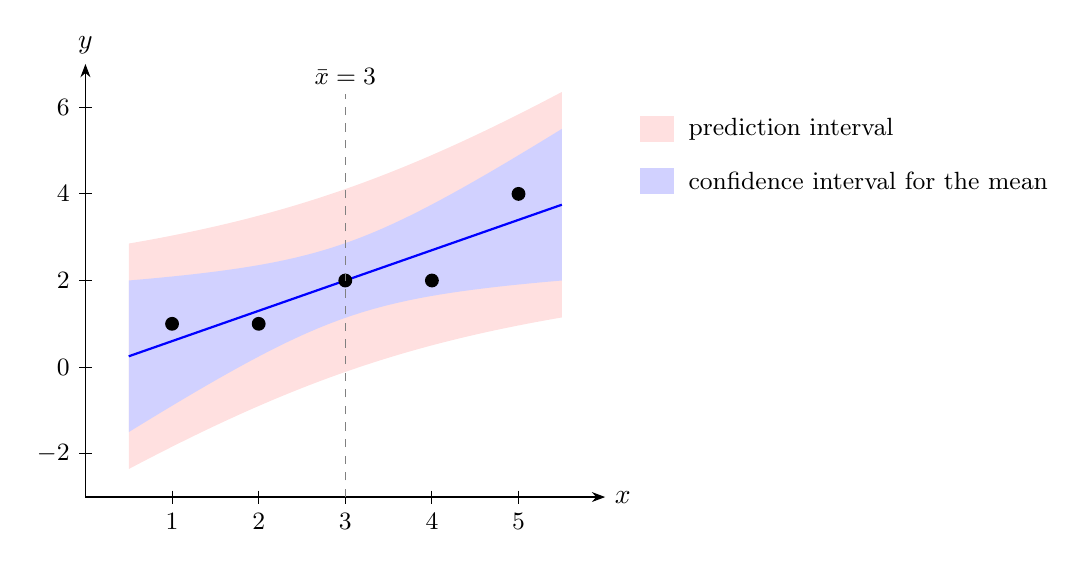
\begin{tikzpicture}[x=1.1cm,y=0.55cm]
\fill[red!12] plot[domain=0.5:5.5,samples=40] (\x,{-0.1+0.7*\x+3.1824*sqrt(0.366667*(1.2+(\x-3)^2/10))})
  -- plot[domain=5.5:0.5,samples=40] (\x,{-0.1+0.7*\x-3.1824*sqrt(0.366667*(1.2+(\x-3)^2/10))}) -- cycle;
\fill[blue!18] plot[domain=0.5:5.5,samples=40] (\x,{-0.1+0.7*\x+3.1824*sqrt(0.366667*(0.2+(\x-3)^2/10))})
  -- plot[domain=5.5:0.5,samples=40] (\x,{-0.1+0.7*\x-3.1824*sqrt(0.366667*(0.2+(\x-3)^2/10))}) -- cycle;
\draw[-Stealth] (0,-3) -- (6,-3) node[right] {$x$};
\draw[-Stealth] (0,-3) -- (0,7) node[above] {$y$};
\foreach \x in {1,...,5} \draw (\x,-2.85) -- (\x,-3.15) node[below] {\small $\x$};
\foreach \y in {-2,0,2,4,6} \draw (0.07,\y) -- (-0.07,\y) node[left] {\small $\y$};
\draw[thick,blue] (0.5,0.25) -- (5.5,3.75);
\foreach \p in {(1,1),(2,1),(3,2),(4,2),(5,4)} \fill \p circle (2.5pt);
\draw[dashed,gray] (3,-3) -- (3,6.3) node[above,black] {\small $\bar x = 3$};
\fill[red!12] (6.4,5.2) rectangle +(0.4,0.6); \node[right] at (6.85,5.5) {\small prediction interval};
\fill[blue!18] (6.4,4.0) rectangle +(0.4,0.6); \node[right] at (6.85,4.3) {\small confidence interval for the mean};
\end{tikzpicture}
\caption{95\% confidence band for the mean response (inner) and prediction band for a new
observation (outer), for the advertising data. Both are narrowest at $\bar x$.}
\label{fig:bands}
\end{figure}

\begin{exa}
For the yield data of Example~\ref{exa:yield}, test significance of regression at the 5\%
level and give a 95\% prediction interval for the yield of a new batch at $45^\circ$C.
\end{exa}

\begin{solution}
Here $\hat\sigma^2 = 0.4762$ with $4$ degrees of freedom, and $t_{0.025,4} = 2.776$.
The standard error of the slope is
$\operatorname{se}(\hat\beta_1) = \sqrt{0.4762/1750} = 0.01650$, so
$t_0 = 0.5714/0.01650 = 34.64$, far beyond $2.776$: the regression is highly significant.

At $x_0 = 45$, $\hat y_0 = 72.048$ and
$1 + \frac16 + \frac{(45 - 35)^2}{1750} = 1.2238$, so
\begin{align*}
72.048 \pm 2.776 \sqrt{0.4762 \times 1.2238} &= 72.048 \pm 2.776 \times 0.7634 \\
&= 72.048 \pm 2.119 ,
\end{align*}
that is, $(69.93,\ 74.17)\%$.
\end{solution}

\subsection{Correlation}\label{ssec:corr}
In regression, $x$ is fixed and $y$ is random. When both are random, measured together on
each unit, their linear association is measured by the correlation coefficient.

\begin{defn}
The \textbf{sample correlation coefficient} is
\[
r = \frac{S_{xy}}{\sqrt{S_{xx} S_{yy}}} .
\]
\end{defn}

By the Cauchy--Schwarz inequality (Problem~\ref{prob:xony}), $-1 \le r \le 1$.
It estimates the population correlation $\rho$.

\begin{thm}\label{thm:r2-r}
\begin{enumerate}[label=(\roman*)]
\item $R^2 = r^2 = \dfrac{S_{xy}^2}{S_{xx} S_{yy}}$;
\item $\hat\beta_1 = r \sqrt{S_{yy}/S_{xx}}$, so $\hat\beta_1$ and $r$ have the same sign;
\item the $t$ statistic for $H_0\colon \beta_1 = 0$ can be written
$t_0 = \dfrac{r\sqrt{n-2}}{\sqrt{1 - r^2}}$.
\end{enumerate}
\end{thm}

\begin{proof}
(i) $R^2 = SS_R/SS_T = \hat\beta_1 S_{xy}/S_{yy} = S_{xy}^2/(S_{xx} S_{yy}) = r^2$.

(ii) $r\sqrt{S_{yy}/S_{xx}} = \dfrac{S_{xy}}{\sqrt{S_{xx}S_{yy}}} \cdot \dfrac{\sqrt{S_{yy}}}{\sqrt{S_{xx}}} = \dfrac{S_{xy}}{S_{xx}} = \hat\beta_1$.

(iii) By (i), $SS_{\mathrm{Res}} = SS_T(1 - R^2) = S_{yy}(1 - r^2)$, so
$\hat\sigma^2 = S_{yy}(1 - r^2)/(n-2)$. Using (ii),
\[
t_0 = \frac{\hat\beta_1}{\sqrt{\hat\sigma^2/S_{xx}}}
= \frac{r\sqrt{S_{yy}/S_{xx}}\, \sqrt{S_{xx}}\, \sqrt{n-2}}{\sqrt{S_{yy}(1 - r^2)}}
= \frac{r\sqrt{n-2}}{\sqrt{1 - r^2}} . \qedhere
\]
\end{proof}

When $x$ and $y$ are jointly normal, (iii) is the test of $H_0\colon \rho = 0$: under $H_0$ it
has the $t_{n-2}$ distribution. So testing for zero correlation and testing for zero slope are
the same test.

\begin{exa}
Find $r$ for the advertising data and test $H_0\colon \rho = 0$ at the 5\% level.
\end{exa}

\begin{solution}
$r = 7/\sqrt{10 \times 6} = 7/\sqrt{60} = 0.9037$, and $r^2 = 0.8167 = R^2$. Then
\[
t_0 = \frac{0.9037\sqrt{3}}{\sqrt{1 - 0.8167}} = \frac{1.5652}{0.4282} = 3.656 ,
\]
the same value as in Example~\ref{exa:disney-test}. As $3.656 > t_{0.025,3} = 3.182$, reject
$H_0$: the correlation is significant.
\end{solution}

\begin{remark}
Correlation measures \emph{linear} association only. Points lying exactly on the parabola
$y = x^2$ for $x = -2, -1, 0, 1, 2$ have $S_{xy} = \sum x_i^3 - n\bar x \bar y = 0$, so $r = 0$,
though $y$ is completely determined by $x$.
\end{remark}

\subsection{Practice problems}
Try each problem before reading the solution.

\begin{problem}\label{prob:fit}
The following data were collected:
\begin{center}
\begin{tabular}{l|ccccc}
$x$ & 2 & 4 & 6 & 8 & 10 \\
\hline
$y$ & 3 & 7 & 8 & 12 & 15 \\
\end{tabular}
\end{center}
\begin{enumerate}[label=(\alph*)]
\item Fit the least-squares line.
\item Compute the fitted values and residuals, and check that $\sum e_i = 0$ and $\sum x_i e_i = 0$.
\item Estimate $\sigma^2$ in two ways, and find $\operatorname{se}(\hat\beta_1)$.
\end{enumerate}
\end{problem}

\begin{solution}
(a) $\sum x_i = 30$, $\sum y_i = 45$, $\sum x_i^2 = 220$, $\sum x_i y_i = 328$, $\sum y_i^2 = 491$,
so $\bar x = 6$ and $\bar y = 9$. Then
\[
S_{xx} = 220 - \frac{30^2}{5} = 40, \qquad S_{xy} = 328 - \frac{30 \times 45}{5} = 58,
\]
$\hat\beta_1 = 58/40 = 1.45$, $\hat\beta_0 = 9 - 1.45 \times 6 = 0.3$, and $\hat y = 0.3 + 1.45x$.

(b)
\begin{center}
\begin{tabular}{c|ccccc}
$x_i$ & 2 & 4 & 6 & 8 & 10 \\
\hline
$\hat y_i$ & 3.2 & 6.1 & 9.0 & 11.9 & 14.8 \\
$e_i$ & $-0.2$ & 0.9 & $-1.0$ & 0.1 & 0.2 \\
\end{tabular}
\end{center}
$\sum e_i = -0.2 + 0.9 - 1.0 + 0.1 + 0.2 = 0$ and
$\sum x_i e_i = -0.4 + 3.6 - 6.0 + 0.8 + 2.0 = 0$.

(c) Directly, $SS_{\mathrm{Res}} = 0.04 + 0.81 + 1.00 + 0.01 + 0.04 = 1.90$. By
Theorem~\ref{thm:ssres}, $S_{yy} = 491 - 45^2/5 = 86$ and
$SS_{\mathrm{Res}} = 86 - 1.45 \times 58 = 86 - 84.1 = 1.90$. So
$\hat\sigma^2 = 1.90/3 = 0.6333$ and $\operatorname{se}(\hat\beta_1) = \sqrt{0.6333/40} = 0.1258$.
\end{solution}

\begin{problem}\label{prob:totals}
For a sample of $n = 10$ weeks, $x$ is advertising spend (in hundreds of dollars) and $y$ is
sales (in thousands of units). Only the totals were kept:
\begin{gather*}
\sum x_i = 50, \quad \sum y_i = 120, \quad \sum x_i^2 = 310, \\
\sum x_i y_i = 660, \quad \sum y_i^2 = 1550 .
\end{gather*}
Find the fitted line, estimate the mean sales when $\$600$ is spent, and estimate $\sigma.$
\end{problem}

\begin{solution}
$\bar x = 5$, $\bar y = 12$, $S_{xx} = 310 - 50^2/10 = 60$, $S_{xy} = 660 - 50 \times 120/10 = 60$
and $S_{yy} = 1550 - 120^2/10 = 110$. So $\hat\beta_1 = 60/60 = 1$, $\hat\beta_0 = 12 - 1 \times 5 = 7$,
and $\hat y = 7 + x$.

$\$600$ is $x = 6$, so $\hat y = 13$, that is, $13\,000$ units.

$SS_{\mathrm{Res}} = 110 - 1 \times 60 = 50$, $\hat\sigma^2 = 50/8 = 6.25$, and
$\hat\sigma = 2.5$ thousand units. Note that the residuals themselves were never needed:
Theorem~\ref{thm:ssres} works from the totals alone.
\end{solution}

\begin{problem}\label{prob:origin}
\textbf{Regression through the origin.} Sometimes theory says the line must pass through the origin, giving the model
$y_i = \beta_1 x_i + \varepsilon_i$.
\begin{enumerate}[label=(\alph*)]
\item Show that the least-squares estimator is $\hat\beta_1 = \sum x_i y_i \big/ \sum x_i^2$.
\item Under A1--A3, show that $\hat\beta_1$ is unbiased with variance $\sigma^2 \big/ \sum x_i^2$.
\item Fit the model to the data below, and show that here $\sum e_i \neq 0$ but $\sum x_i e_i = 0$.
\end{enumerate}
\begin{center}
\begin{tabular}{l|cccccc}
$x$ & 1 & 2 & 3 & 4 & 5 & 6 \\
\hline
$y$ & 2.1 & 3.9 & 6.2 & 7.8 & 10.1 & 11.9 \\
\end{tabular}
\end{center}
\end{problem}

\begin{solution}
(a) $S(\beta_1) = \sum (y_i - \beta_1 x_i)^2$ has
$S'(\beta_1) = -2\sum x_i (y_i - \beta_1 x_i)$. Setting this to zero gives
$\sum x_i y_i = \hat\beta_1 \sum x_i^2$. Since $S''(\beta_1) = 2\sum x_i^2 > 0$, this is a
minimum.

(b) $\hat\beta_1 = \sum k_i y_i$ with $k_i = x_i / \sum x_j^2$. Then
$E(\hat\beta_1) = \sum k_i \beta_1 x_i = \beta_1 \sum x_i^2 / \sum x_j^2 = \beta_1$, and
$\operatorname{Var}(\hat\beta_1) = \sigma^2 \sum k_i^2 = \sigma^2 \sum x_i^2 / \left(\sum x_j^2\right)^2 = \sigma^2 / \sum x_i^2$.

(c) $\sum x_i y_i = 2.1 + 7.8 + 18.6 + 31.2 + 50.5 + 71.4 = 181.6$ and $\sum x_i^2 = 91$, so
$\hat\beta_1 = 181.6/91 = 1.9956$ and $\hat y = 1.9956x$. Then
\begin{align*}
\sum e_i &= \sum y_i - \hat\beta_1 \sum x_i = 42 - 1.9956 \times 21 \\
         &= 42 - 41.9077 = 0.0923 \neq 0 ,
\end{align*}
while $\sum x_i e_i = \sum x_i y_i - \hat\beta_1 \sum x_i^2 = 181.6 - 181.6 = 0$.
The only normal equation is the one for $\beta_1$, which is $\sum x_i e_i = 0$. The equation
that gave $\sum e_i = 0$ belonged to $\beta_0$, and this model has no $\beta_0$.
\end{solution}

\begin{problem}\label{prob:xony}
For the advertising data, fit the regression of $x$ on $y$, that is, the line
$\hat x = \hat\alpha_0 + \hat\alpha_1 y$ that minimises $\sum (x_i - \alpha_0 - \alpha_1 y_i)^2$.
Is it the same line as $\hat y = -0.1 + 0.7x$ solved for $x$? Show that in general the
product of the two slopes, $\hat\beta_1 \hat\alpha_1$, lies between $0$ and $1$.
\end{problem}

\begin{solution}
By Theorem~\ref{thm:ls} with the roles of $x$ and $y$ exchanged,
$\hat\alpha_1 = S_{xy}/S_{yy} = 7/6 = 1.1667$ and
$\hat\alpha_0 = \bar x - \hat\alpha_1 \bar y = 3 - (7/6)(2) = 0.6667$.

Solving $\hat y = -0.1 + 0.7x$ for $x$ gives $x = (y + 0.1)/0.7$, with slope
$1/0.7 = 1.4286$. The two lines are different: one minimises vertical distances, the other
horizontal ones.

In general
\[
\hat\beta_1 \hat\alpha_1 = \frac{S_{xy}}{S_{xx}} \cdot \frac{S_{xy}}{S_{yy}} = \frac{S_{xy}^2}{S_{xx} S_{yy}} \ge 0 .
\]
By the Cauchy--Schwarz inequality,
$\left( \sum a_i b_i \right)^2 \le \sum a_i^2 \sum b_i^2$. With $a_i = x_i - \bar x$ and
$b_i = y_i - \bar y$ this says $S_{xy}^2 \le S_{xx} S_{yy}$, so the product is at most $1$.
It equals $1$ exactly when the points lie on a straight line, and only then do the two
regression lines coincide. Here $\hat\beta_1 \hat\alpha_1 = 49/60 = 0.8167$. This quantity
is $r^2$, the square of the correlation coefficient of Subsection~\ref{ssec:corr}.
\end{solution}

\begin{problem}\label{prob:full}
Continue with the data of Problem~\ref{prob:fit}, assuming A1--A4.
\begin{enumerate}[label=(\alph*)]
\item Test $H_0\colon \beta_1 = 0$ against $H_1\colon \beta_1 \neq 0$ at the 5\% level, using the $t$-test.
\item Set out the analysis of variance table, carry out the $F$-test, and check that $F_0 = t_0^2$.
\item Find $R^2$ and the correlation coefficient $r$.
\item Find a 95\% confidence interval for $\beta_1$.
\item At $x_0 = 7$, find a 95\% confidence interval for the mean response and a 95\% prediction interval for a new observation.
\end{enumerate}
\end{problem}

\begin{solution}
From Problem~\ref{prob:fit}: $n = 5$, $\bar x = 6$, $S_{xx} = 40$, $S_{xy} = 58$,
$S_{yy} = 86$, $\hat\beta_1 = 1.45$, $\hat\beta_0 = 0.3$, $SS_{\mathrm{Res}} = 1.90$,
$\hat\sigma^2 = 0.6333$ and $\operatorname{se}(\hat\beta_1) = 0.1258$. There are $n - 2 = 3$
degrees of freedom, and $t_{0.025,3} = 3.182$.

(a) $t_0 = 1.45/0.1258 = 11.52$. Since $|t_0| > 3.182$, reject $H_0$: there is a significant
linear relationship.

(b) $SS_R = \hat\beta_1 S_{xy} = 1.45 \times 58 = 84.1$.
\begin{center}
\begin{tabular}{lcccc}
\hline
Source & SS & df & MS & $F_0$ \\
\hline
Regression & 84.10 & 1 & 84.10 & 132.79 \\
Residual & 1.90 & 3 & 0.6333 & \\
\hline
Total & 86.00 & 4 & & \\
\hline
\end{tabular}
\end{center}
$F_{0.05,1,3} = 10.13$, and $132.79 > 10.13$, so reject $H_0$. Also
$t_0^2 = 11.523^2 = 132.79 = F_0$.

(c) $R^2 = 84.1/86 = 0.9779$, so the line explains about $97.8\%$ of the variation in $y$.
$r = +\sqrt{0.9779} = 0.9889$, positive because $S_{xy} > 0$.

(d) $1.45 \pm 3.182 \times 0.1258 = 1.45 \pm 0.4004$, that is, $(1.0496,\ 1.8504)$.

(e) $\hat y_0 = 0.3 + 1.45 \times 7 = 10.45$, and
$\frac1n + \frac{(x_0 - \bar x)^2}{S_{xx}} = 0.2 + \frac{1}{40} = 0.225$.
\begin{itemize}
\item Mean response: standard error $\sqrt{0.6333 \times 0.225} = 0.3775$; interval
$10.45 \pm 3.182 \times 0.3775 = 10.45 \pm 1.201$, that is, $(9.249,\ 11.651)$.
\item New observation: standard error $\sqrt{0.6333 \times 1.225} = 0.8808$; interval
$10.45 \pm 3.182 \times 0.8808 = 10.45 \pm 2.803$, that is, $(7.647,\ 13.253)$.
\end{itemize}
\end{solution}

\begin{problem}
For the advertising totals of Problem~\ref{prob:totals} ($n = 10$, $\hat y = 7 + x$, $S_{xx} = 60$,
$S_{yy} = 110$, $\hat\sigma^2 = 6.25$):
\begin{enumerate}[label=(\alph*)]
\item test at the 5\% level whether sales are linearly related to advertising;
\item a manager claims that each extra $\$100$ of advertising raises mean sales by more than
$500$ units. Test $H_0\colon \beta_1 = 0.5$ against $H_1\colon \beta_1 > 0.5$ at the 5\% level;
\item find a 95\% confidence interval for $\sigma^2$.
\end{enumerate}
\end{problem}

\begin{solution}
There are $n - 2 = 8$ degrees of freedom, and
$\operatorname{se}(\hat\beta_1) = \sqrt{6.25/60} = 0.3227$.

(a) $t_0 = 1/0.3227 = 3.098 > t_{0.025,8} = 2.306$: reject $H_0\colon \beta_1 = 0$. Sales are
significantly related to advertising.

(b) $t_0 = (1 - 0.5)/0.3227 = 1.549$. The test is one-sided, so the critical value is
$t_{0.05,8} = 1.860$. As $1.549 < 1.860$ we do not reject $H_0$: the data do not support the
manager's claim, even though the estimate $\hat\beta_1 = 1$ is above $0.5$. The estimate is
too imprecise for that.

(c) $SS_{\mathrm{Res}} = 50$, $\chi^2_{0.025,8} = 17.535$ and $\chi^2_{0.975,8} = 2.180$, so
the interval is
\[
\left( \frac{50}{17.535},\ \frac{50}{2.180} \right) = (2.85,\ 22.94) .
\]
It is very wide: eight degrees of freedom tell us little about a variance.
\end{solution}

\begin{problem}
\begin{enumerate}[label=(\alph*)]
\item Show that the confidence interval for the mean response is narrowest at $x_0 = \bar x$,
and that the prediction interval at any $x_0$ is wider than the confidence interval there.
\item As $n \to \infty$, with the $x_i$ spread so that $S_{xx} \to \infty$ and $\bar x$ stays
bounded, what happens to the width of each interval?
\end{enumerate}
\end{problem}

\begin{solution}
(a) The half-width of the confidence interval is
$t_{\alpha/2,n-2} \sqrt{\hat\sigma^2 \bigl( \frac1n + \frac{(x_0 - \bar x)^2}{S_{xx}} \bigr)}$.
Only $(x_0 - \bar x)^2$ depends on $x_0$, and it is least, namely $0$, at $x_0 = \bar x$.
The prediction interval has $1 + \frac1n + \frac{(x_0 - \bar x)^2}{S_{xx}}$ under the
square root in place of $\frac1n + \frac{(x_0 - \bar x)^2}{S_{xx}}$, which is larger by $1$,
with the same $t$ and $\hat\sigma^2$.

(b) $\frac1n \to 0$ and $\frac{(x_0 - \bar x)^2}{S_{xx}} \to 0$, while $\hat\sigma^2 \to \sigma^2$
and $t_{\alpha/2,n-2} \to z_{\alpha/2}$. So the confidence interval shrinks to the single point
$E(y \mid x_0)$: with enough data the line is known exactly. The prediction interval tends to
$E(y \mid x_0) \pm z_{\alpha/2}\sigma$, which does not shrink. However well the line is known,
a new observation still carries its own error $\varepsilon_0$.
\end{solution}

\begin{problem}
Show that $R^2$ is unchanged if every $y_i$ is replaced by $a + b y_i$ and every $x_i$ by
$c + d x_i$, where $b \neq 0$ and $d \neq 0$. What happens to $\hat\beta_1$?
\end{problem}

\begin{solution}
Write $u_i = c + d x_i$ and $v_i = a + b y_i$. Then $\bar u = c + d\bar x$, so
$u_i - \bar u = d(x_i - \bar x)$, and similarly $v_i - \bar v = b(y_i - \bar y)$. Hence
\[
S_{uu} = d^2 S_{xx}, \qquad S_{vv} = b^2 S_{yy}, \qquad S_{uv} = bd\, S_{xy},
\]
and by Theorem~\ref{thm:r2-r},
\[
R^2_{\text{new}} = \frac{S_{uv}^2}{S_{uu} S_{vv}} = \frac{b^2 d^2 S_{xy}^2}{d^2 S_{xx}\, b^2 S_{yy}} = \frac{S_{xy}^2}{S_{xx} S_{yy}} = R^2 .
\]
The slope becomes $S_{uv}/S_{uu} = (b/d)\hat\beta_1$. Changing the units changes the slope
but not how well the line fits. Measuring sales in thousands of units instead of units, for
instance, divides $\hat\beta_1$ by $1000$ and leaves $R^2$ alone.
\end{solution}






\section{Multiple linear regression}
Most responses depend on more than one variable. Crop yield depends on fertiliser and on
rainfall; the time to make a delivery depends on the number of items and on the distance.
A \textbf{multiple linear regression model} with $k$ regressors is
\begin{equation}\label{eq:mlr}
y = \beta_0 + \beta_1 x_1 + \beta_2 x_2 + \cdots + \beta_k x_k + \varepsilon .
\end{equation}
It has $p = k + 1$ parameters $\beta_0, \beta_1, \dots, \beta_k$, called the
\textbf{regression coefficients}.

\begin{remark}
$\beta_j$ is the change in the mean response $E(y)$ per unit increase in $x_j$
\emph{when all the other regressors are held fixed}. For this reason the $\beta_j$ are
called \textbf{partial regression coefficients}. With one regressor, $E(y)$ is a line; with
two it is a plane, as in Figure~\ref{fig:plane}; with more it is a \emph{hyperplane}, which
cannot be drawn but is handled in exactly the same way.
\end{remark}

As in the last section, ``linear'' refers to the parameters. A model such as
$y = \beta_0 + \beta_1 x + \beta_2 x^2 + \varepsilon$ is a multiple linear regression model
with $x_1 = x$ and $x_2 = x^2$, and everything in this section applies to it.

Multiple regression is carried out with matrices. The formulas of simple linear regression
were already long with one regressor; written out term by term for $k$ regressors they would
be unmanageable. In matrix form, one formula covers every $k$, and simple linear regression
becomes the special case $k = 1$.

\subsection{Matrix results we shall need}
Vectors are columns and are printed in bold: $\mathbf{y}$, $\boldsymbol\beta$. The
transpose of $\mathbf{A}$ is $\mathbf{A}^\top$, and $(\mathbf{AB})^\top = \mathbf{B}^\top \mathbf{A}^\top$.
The \textbf{trace} of a square matrix is the sum of its diagonal entries,
$\operatorname{tr}(\mathbf{A}) = \sum_i a_{ii}$.

\begin{lem}[Trace]\label{lem:trace}
If $\mathbf{A}$ is $m \times n$ and $\mathbf{B}$ is $n \times m$, then
$\operatorname{tr}(\mathbf{AB}) = \operatorname{tr}(\mathbf{BA})$.
\end{lem}

\begin{proof}
$\operatorname{tr}(\mathbf{AB}) = \sum_{i=1}^m (\mathbf{AB})_{ii} = \sum_{i=1}^m \sum_{j=1}^n a_{ij} b_{ji}$
and $\operatorname{tr}(\mathbf{BA}) = \sum_{j=1}^n \sum_{i=1}^m b_{ji} a_{ij}$. These are the
same sum taken in a different order.
\end{proof}

\begin{lem}[Differentiation]\label{lem:diff}
For a vector $\boldsymbol\beta = (\beta_0, \dots, \beta_k)^\top$, let
$\partial f / \partial \boldsymbol\beta$ denote the vector of partial derivatives
$\partial f / \partial \beta_j$. Then, for a constant vector $\mathbf{a}$ and a constant
symmetric matrix $\mathbf{A}$,
\[
\frac{\partial (\mathbf{a}^\top \boldsymbol\beta)}{\partial \boldsymbol\beta} = \mathbf{a},
\qquad
\frac{\partial (\boldsymbol\beta^\top \mathbf{A} \boldsymbol\beta)}{\partial \boldsymbol\beta} = 2\mathbf{A}\boldsymbol\beta .
\]
\end{lem}

\begin{proof}
$\mathbf{a}^\top \boldsymbol\beta = \sum_j a_j \beta_j$, whose derivative with respect to
$\beta_m$ is $a_m$. Next,
\[
\boldsymbol\beta^\top \mathbf{A} \boldsymbol\beta = \sum_i \sum_j a_{ij} \beta_i \beta_j .
\]
Differentiating with respect to $\beta_m$, the terms with $i = m$ give $\sum_j a_{mj}\beta_j$
and the terms with $j = m$ give $\sum_i a_{im}\beta_i$. Since $a_{im} = a_{mi}$, both equal
the $m$th entry of $\mathbf{A}\boldsymbol\beta$, so the derivative is
$2(\mathbf{A}\boldsymbol\beta)_m$.
\end{proof}

For a random vector $\mathbf{y} = (y_1, \dots, y_n)^\top$, the \textbf{mean vector}
$E(\mathbf{y})$ has entries $E(y_i)$, and the \textbf{covariance matrix}
\[
\operatorname{Var}(\mathbf{y}) = E\left[ (\mathbf{y} - E\mathbf{y})(\mathbf{y} - E\mathbf{y})^\top \right]
\]
has $(i,j)$ entry $\operatorname{Cov}(y_i, y_j)$, and so has the variances
$\operatorname{Var}(y_i)$ down its diagonal.

\begin{lem}[Linear functions of a random vector]\label{lem:linear-rv}
If $\mathbf{A}$ is a constant matrix and $\mathbf{b}$ a constant vector, then
\[
E(\mathbf{A}\mathbf{y} + \mathbf{b}) = \mathbf{A}E(\mathbf{y}) + \mathbf{b},
\qquad
\operatorname{Var}(\mathbf{A}\mathbf{y} + \mathbf{b}) = \mathbf{A} \operatorname{Var}(\mathbf{y}) \mathbf{A}^\top .
\]
\end{lem}

\begin{proof}
The $i$th entry of $\mathbf{Ay} + \mathbf{b}$ is $\sum_j a_{ij} y_j + b_i$, whose expectation
is $\sum_j a_{ij} E(y_j) + b_i$, the $i$th entry of $\mathbf{A}E(\mathbf{y}) + \mathbf{b}$.
Writing $\boldsymbol\mu = E(\mathbf{y})$, we have
$\mathbf{Ay} + \mathbf{b} - E(\mathbf{Ay} + \mathbf{b}) = \mathbf{A}(\mathbf{y} - \boldsymbol\mu)$, so
\[
\operatorname{Var}(\mathbf{Ay} + \mathbf{b})
= E\left[ \mathbf{A}(\mathbf{y} - \boldsymbol\mu)(\mathbf{y} - \boldsymbol\mu)^\top \mathbf{A}^\top \right]
= \mathbf{A} \operatorname{Var}(\mathbf{y}) \mathbf{A}^\top ,
\]
taking the constant matrices outside the expectation.
\end{proof}

\begin{lem}[Expected quadratic form]\label{lem:quad-form}
If $E(\mathbf{y}) = \boldsymbol\mu$, $\operatorname{Var}(\mathbf{y}) = \mathbf{V}$ and
$\mathbf{A}$ is a constant matrix, then
\[
E(\mathbf{y}^\top \mathbf{A} \mathbf{y}) = \operatorname{tr}(\mathbf{AV}) + \boldsymbol\mu^\top \mathbf{A} \boldsymbol\mu .
\]
\end{lem}

\begin{proof}
Write $\mathbf{y} = \boldsymbol\mu + \mathbf{z}$, where $E(\mathbf{z}) = \mathbf{0}$ and
$E(\mathbf{z}\mathbf{z}^\top) = \mathbf{V}$. Then
\[
\mathbf{y}^\top \mathbf{A} \mathbf{y}
= \boldsymbol\mu^\top \mathbf{A} \boldsymbol\mu + \boldsymbol\mu^\top \mathbf{A} \mathbf{z}
  + \mathbf{z}^\top \mathbf{A} \boldsymbol\mu + \mathbf{z}^\top \mathbf{A} \mathbf{z} .
\]
The two middle terms have expectation $0$. The last is a $1 \times 1$ matrix, so equals its
own trace, and by Lemma~\ref{lem:trace}
$\mathbf{z}^\top \mathbf{A} \mathbf{z} = \operatorname{tr}(\mathbf{z}^\top \mathbf{A} \mathbf{z}) = \operatorname{tr}(\mathbf{A} \mathbf{z}\mathbf{z}^\top)$.
Since the trace is a sum of entries, it can be taken through the expectation:
$E\operatorname{tr}(\mathbf{A}\mathbf{z}\mathbf{z}^\top) = \operatorname{tr}(\mathbf{A}\,E(\mathbf{z}\mathbf{z}^\top)) = \operatorname{tr}(\mathbf{AV})$.
\end{proof}

Finally, from linear algebra: a square matrix $\mathbf{A}$ has an inverse exactly when
$\det \mathbf{A} \neq 0$, and then
\[
\mathbf{A}^{-1} = \frac{1}{\det \mathbf{A}} \operatorname{adj}(\mathbf{A}),
\]
where the \textbf{adjugate} $\operatorname{adj}(\mathbf{A})$ is the transpose of the matrix
of cofactors. The cofactor of $a_{ij}$ is $(-1)^{i+j}$ times the determinant of the matrix
left when row $i$ and column $j$ are deleted. For a symmetric matrix, such as the ones met
in regression, the matrix of cofactors is itself symmetric and no transposing is needed.

\subsection{The model in matrix form}
For a sample of $n$ observations, the model~\eqref{eq:mlr} says
$y_i = \beta_0 + \beta_1 x_{i1} + \cdots + \beta_k x_{ik} + \varepsilon_i$, for
$i = 1, \dots, n$, where $x_{ij}$ is the value of the $j$th regressor in the $i$th
observation. Stack these $n$ equations:
\[
\underbrace{\begin{bmatrix} y_1 \\ y_2 \\ \vdots \\ y_n \end{bmatrix}}_{\mathbf{y}}
=
\underbrace{\begin{bmatrix}
1 & x_{11} & \cdots & x_{1k} \\
1 & x_{21} & \cdots & x_{2k} \\
\vdots & \vdots & & \vdots \\
1 & x_{n1} & \cdots & x_{nk}
\end{bmatrix}}_{\mathbf{X}}
\underbrace{\begin{bmatrix} \beta_0 \\ \beta_1 \\ \vdots \\ \beta_k \end{bmatrix}}_{\boldsymbol\beta}
+
\underbrace{\begin{bmatrix} \varepsilon_1 \\ \varepsilon_2 \\ \vdots \\ \varepsilon_n \end{bmatrix}}_{\boldsymbol\varepsilon},
\]
that is,
\[
\boxed{\;\mathbf{y} = \mathbf{X}\boldsymbol\beta + \boldsymbol\varepsilon\;}
\]
The $n \times p$ matrix $\mathbf{X}$ is the \textbf{model matrix} (or design matrix). Its
first column of ones carries the intercept, and each further column holds the values of one
regressor.

The assumptions A1--A4 of simple regression become:
\begin{enumerate}[label=\textbf{A\arabic*.}]
\item $E(\boldsymbol\varepsilon) = \mathbf{0}$;
\item[\textbf{A2--3.}] $\operatorname{Var}(\boldsymbol\varepsilon) = \sigma^2 \mathbf{I}$: the
diagonal says every error has variance $\sigma^2$, the zeros off the diagonal say the errors
are uncorrelated;
\setcounter{enumi}{3}
\item $\boldsymbol\varepsilon \sim N_n(\mathbf{0}, \sigma^2\mathbf{I})$: the errors are
independent normal variables.
\end{enumerate}
We also assume that $\mathbf{X}$ has \textbf{full column rank} $p$: no column is a linear
combination of the others. This is the analogue of ``the $x_i$ are not all equal'' in simple
regression. By Lemma~\ref{lem:linear-rv}, A1--A3 give
$E(\mathbf{y}) = \mathbf{X}\boldsymbol\beta$ and $\operatorname{Var}(\mathbf{y}) = \sigma^2\mathbf{I}$.

\begin{exa}\label{exa:crop}
An agronomist records the yield $y$ (tonnes per hectare) on six plots, with the fertiliser
applied, $x_1$ (in 100\,kg per hectare), and the rainfall, $x_2$ (in 100\,mm):
\begin{center}
\begin{tabular}{c|cccccc}
Plot & 1 & 2 & 3 & 4 & 5 & 6 \\
\hline
Fertiliser $x_1$ & 1 & 2 & 2 & 3 & 4 & 6 \\
Rainfall $x_2$ & 2 & 1 & 3 & 2 & 4 & 3 \\
Yield $y$ & 6 & 9 & 11 & 10 & 15 & 18 \\
\end{tabular}
\end{center}
For the model $y = \beta_0 + \beta_1 x_1 + \beta_2 x_2 + \varepsilon$, $n = 6$, $k = 2$,
$p = 3$, and
\[
\mathbf{y} = \begin{bmatrix} 6 \\ 9 \\ 11 \\ 10 \\ 15 \\ 18 \end{bmatrix}, \qquad
\mathbf{X} = \begin{bmatrix}
1 & 1 & 2 \\ 1 & 2 & 1 \\ 1 & 2 & 3 \\ 1 & 3 & 2 \\ 1 & 4 & 4 \\ 1 & 6 & 3
\end{bmatrix} .
\]
\end{exa}

\subsection{Least-squares estimation}
The least-squares criterion is again the sum of squared errors, now written
\[
S(\boldsymbol\beta) = \sum_{i=1}^n \varepsilon_i^2 = \boldsymbol\varepsilon^\top \boldsymbol\varepsilon
= (\mathbf{y} - \mathbf{X}\boldsymbol\beta)^\top (\mathbf{y} - \mathbf{X}\boldsymbol\beta) .
\]

\begin{thm}[Least-squares estimator]\label{thm:ls-matrix}
If $\mathbf{X}$ has full column rank, $\mathbf{X}^\top \mathbf{X}$ is invertible and the
unique least-squares estimator of $\boldsymbol\beta$ is
\[
\boxed{\;\hat{\boldsymbol\beta} = (\mathbf{X}^\top \mathbf{X})^{-1} \mathbf{X}^\top \mathbf{y}\;}
\]
It is the solution of the \textbf{normal equations}
$\mathbf{X}^\top \mathbf{X} \hat{\boldsymbol\beta} = \mathbf{X}^\top \mathbf{y}$.
\end{thm}

\begin{proof}
\emph{$\mathbf{X}^\top\mathbf{X}$ is invertible.} If $\mathbf{X}^\top\mathbf{X}\mathbf{v} = \mathbf{0}$
then $0 = \mathbf{v}^\top \mathbf{X}^\top \mathbf{X} \mathbf{v} = (\mathbf{Xv})^\top (\mathbf{Xv}) = \sum_i (\mathbf{Xv})_i^2$,
so $\mathbf{Xv} = \mathbf{0}$. Full column rank means this happens only for
$\mathbf{v} = \mathbf{0}$. So the square matrix $\mathbf{X}^\top\mathbf{X}$ sends no
non-zero vector to zero, and is invertible.

\emph{The stationary point.} Expanding, and using the fact that the $1\times1$ matrix
$\boldsymbol\beta^\top \mathbf{X}^\top \mathbf{y}$ equals its transpose $\mathbf{y}^\top \mathbf{X}\boldsymbol\beta$,
\[
S(\boldsymbol\beta) = \mathbf{y}^\top\mathbf{y} - 2\boldsymbol\beta^\top \mathbf{X}^\top \mathbf{y}
  + \boldsymbol\beta^\top \mathbf{X}^\top \mathbf{X} \boldsymbol\beta .
\]
$\mathbf{X}^\top\mathbf{X}$ is symmetric, so by Lemma~\ref{lem:diff}
\[
\frac{\partial S}{\partial \boldsymbol\beta} = -2\mathbf{X}^\top\mathbf{y} + 2\mathbf{X}^\top\mathbf{X}\boldsymbol\beta ,
\]
which is zero exactly when $\mathbf{X}^\top\mathbf{X}\boldsymbol\beta = \mathbf{X}^\top\mathbf{y}$,
that is, at $\hat{\boldsymbol\beta}$.

\emph{It is the minimum.} For any $\boldsymbol\beta$, write
$\mathbf{y} - \mathbf{X}\boldsymbol\beta = (\mathbf{y} - \mathbf{X}\hat{\boldsymbol\beta}) + \mathbf{X}(\hat{\boldsymbol\beta} - \boldsymbol\beta)$.
The cross term vanishes, because
$\mathbf{X}^\top(\mathbf{y} - \mathbf{X}\hat{\boldsymbol\beta}) = \mathbf{X}^\top\mathbf{y} - \mathbf{X}^\top\mathbf{X}\hat{\boldsymbol\beta} = \mathbf{0}$
by the normal equations. Hence
\[
S(\boldsymbol\beta) = S(\hat{\boldsymbol\beta})
  + (\hat{\boldsymbol\beta} - \boldsymbol\beta)^\top \mathbf{X}^\top \mathbf{X} (\hat{\boldsymbol\beta} - \boldsymbol\beta) .
\]
The last term is $\sum_i \bigl(\mathbf{X}(\hat{\boldsymbol\beta} - \boldsymbol\beta)\bigr)_i^2 \ge 0$,
and by the first part it is zero only when $\boldsymbol\beta = \hat{\boldsymbol\beta}$.
So $S(\boldsymbol\beta) > S(\hat{\boldsymbol\beta})$ for every other $\boldsymbol\beta$.
\end{proof}

The entries of $\mathbf{X}^\top\mathbf{X}$ and $\mathbf{X}^\top\mathbf{y}$ are the familiar
sums. With two regressors,
\[
\mathbf{X}^\top\mathbf{X} = \begin{bmatrix}
n & \sum x_{i1} & \sum x_{i2} \\
\sum x_{i1} & \sum x_{i1}^2 & \sum x_{i1}x_{i2} \\
\sum x_{i2} & \sum x_{i1}x_{i2} & \sum x_{i2}^2
\end{bmatrix},
\qquad
\mathbf{X}^\top\mathbf{y} = \begin{bmatrix} \sum y_i \\ \sum x_{i1} y_i \\ \sum x_{i2} y_i \end{bmatrix} .
\]
So the hand calculation starts, as before, with a table of column totals.

\begin{exa}[Simple regression as a special case]\label{exa:slr-matrix}
With one regressor, $\mathbf{X}$ has columns $\mathbf{1}$ and $(x_1, \dots, x_n)^\top$, and
\[
\mathbf{X}^\top\mathbf{X} = \begin{bmatrix} n & \sum x_i \\ \sum x_i & \sum x_i^2 \end{bmatrix},
\]
\[
\det(\mathbf{X}^\top\mathbf{X}) = n\sum x_i^2 - \left(\sum x_i\right)^2 = nS_{xx} .
\]
For a $2 \times 2$ matrix the adjugate swaps the diagonal entries and changes the sign of the
others, so
\[
(\mathbf{X}^\top\mathbf{X})^{-1} = \frac{1}{nS_{xx}} \begin{bmatrix} \sum x_i^2 & -\sum x_i \\ -\sum x_i & n \end{bmatrix} .
\]
The second entry of $\hat{\boldsymbol\beta} = (\mathbf{X}^\top\mathbf{X})^{-1}\mathbf{X}^\top\mathbf{y}$ is
\[
\hat\beta_1 = \frac{n\sum x_i y_i - \sum x_i \sum y_i}{nS_{xx}}
= \frac{\sum x_i y_i - n\bar x \bar y}{S_{xx}} = \frac{S_{xy}}{S_{xx}} ,
\]
the formula of Theorem~\ref{thm:ls}. The first entry gives $\hat\beta_0 = \bar y - \hat\beta_1\bar x$
in the same way (Problem~\ref{prob:slr-matrix}).
\end{exa}

\begin{exa}\label{exa:crop-fit}
Fit the model to the crop data of Example~\ref{exa:crop}.
\end{exa}

\begin{solution}
\emph{Step 1: the sums.}
\begin{center}
\begin{tabular}{c|cccccccc}
$i$ & $x_{i1}$ & $x_{i2}$ & $y_i$ & $x_{i1}^2$ & $x_{i2}^2$ & $x_{i1}x_{i2}$ & $x_{i1}y_i$ & $x_{i2}y_i$ \\
\hline
1 & 1 & 2 & 6 & 1 & 4 & 2 & 6 & 12 \\
2 & 2 & 1 & 9 & 4 & 1 & 2 & 18 & 9 \\
3 & 2 & 3 & 11 & 4 & 9 & 6 & 22 & 33 \\
4 & 3 & 2 & 10 & 9 & 4 & 6 & 30 & 20 \\
5 & 4 & 4 & 15 & 16 & 16 & 16 & 60 & 60 \\
6 & 6 & 3 & 18 & 36 & 9 & 18 & 108 & 54 \\
\hline
$\sum$ & 18 & 15 & 69 & 70 & 43 & 50 & 244 & 188 \\
\end{tabular}
\end{center}
so
\[
\mathbf{X}^\top\mathbf{X} = \begin{bmatrix} 6 & 18 & 15 \\ 18 & 70 & 50 \\ 15 & 50 & 43 \end{bmatrix},
\qquad
\mathbf{X}^\top\mathbf{y} = \begin{bmatrix} 69 \\ 244 \\ 188 \end{bmatrix} .
\]
\emph{Step 2: the cofactors.} Deleting row $i$ and column $j$ and taking the determinant of
what is left:
\begin{align*}
C_{11} &= +(70 \cdot 43 - 50 \cdot 50) = 3010 - 2500 = 510, \\
C_{12} &= -(18 \cdot 43 - 50 \cdot 15) = -(774 - 750) = -24, \\
C_{13} &= +(18 \cdot 50 - 70 \cdot 15) = 900 - 1050 = -150, \\
C_{22} &= +(6 \cdot 43 - 15 \cdot 15) = 258 - 225 = 33, \\
C_{23} &= -(6 \cdot 50 - 18 \cdot 15) = -(300 - 270) = -30, \\
C_{33} &= +(6 \cdot 70 - 18 \cdot 18) = 420 - 324 = 96 ,
\end{align*}
and by symmetry $C_{21} = C_{12}$, $C_{31} = C_{13}$, $C_{32} = C_{23}$.

\emph{Step 3: the determinant}, expanding along the first row:
\[
\det(\mathbf{X}^\top\mathbf{X}) = 6(510) + 18(-24) + 15(-150) = 3060 - 432 - 2250 = 378 .
\]
\emph{Step 4: the inverse.}
\[
(\mathbf{X}^\top\mathbf{X})^{-1} = \frac{1}{378}
\begin{bmatrix} 510 & -24 & -150 \\ -24 & 33 & -30 \\ -150 & -30 & 96 \end{bmatrix} .
\]
A check: the first row of $\mathbf{X}^\top\mathbf{X}$ times the first column of the adjugate
should give $378$, and times the second column $0$:
$6(510) + 18(-24) + 15(-150) = 378$ and $6(-24) + 18(33) + 15(-30) = -144 + 594 - 450 = 0$.

\emph{Step 5: the estimates.}
\[
\hat{\boldsymbol\beta} = \frac{1}{378}
\begin{bmatrix} 510(69) - 24(244) - 150(188) \\ -24(69) + 33(244) - 30(188) \\ -150(69) - 30(244) + 96(188) \end{bmatrix}
= \frac{1}{378} \begin{bmatrix} 1134 \\ 756 \\ 378 \end{bmatrix}
= \begin{bmatrix} 3 \\ 2 \\ 1 \end{bmatrix} .
\]
The fitted model is
\[
\hat y = 3 + 2x_1 + x_2 .
\]
\textbf{Interpretation.} At a fixed rainfall, each extra 100\,kg of fertiliser per hectare
raises the mean yield by $2$ tonnes per hectare; at a fixed fertiliser rate, each extra
100\,mm of rain raises it by $1$ tonne per hectare.
\end{solution}

\begin{figure}[H]
\centering
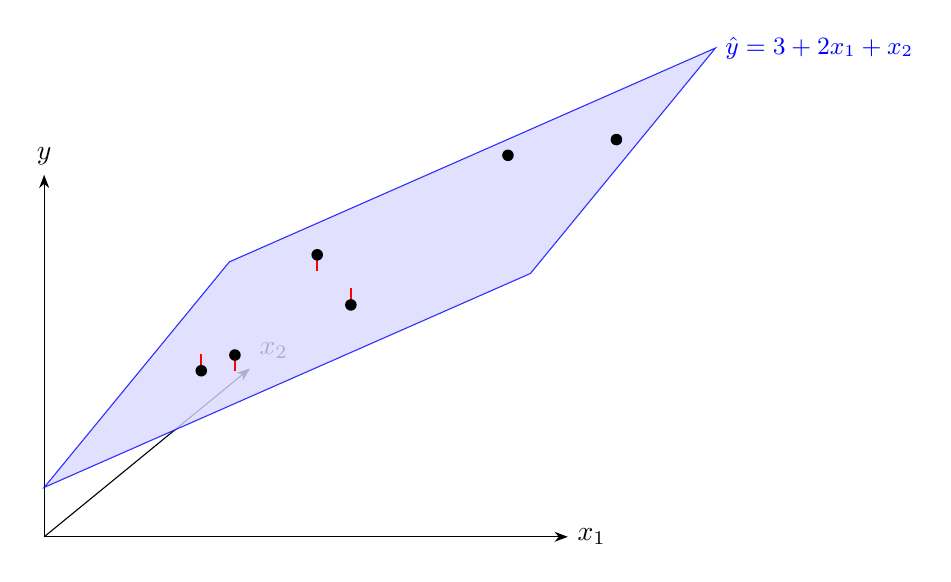
\begin{tikzpicture}[x={(1cm,0cm)},y={(0.55cm,0.45cm)},z={(0cm,0.22cm)},scale=0.95]
\draw[-Stealth] (0,0,0) -- (7,0,0) node[right] {$x_1$};
\draw[-Stealth] (0,0,0) -- (0,5,0) node[above right] {$x_2$};
\draw[-Stealth] (0,0,0) -- (0,0,22) node[above] {$y$};
\filldraw[fill=blue!15,draw=blue,opacity=0.8] (0,0,3) -- (6.5,0,16) -- (6.5,4.5,20.5) -- (0,4.5,7.5) -- cycle;
\foreach \a/\b/\c in {1/2/6,2/1/9,2/3/11,3/2/10,4/4/15,6/3/18} {
  \draw[red,thick] (\a,\b,\c) -- (\a,\b,{3+2*\a+\b});
  \fill (\a,\b,\c) circle (2.2pt);
}
\node[blue,right] at (6.5,4.5,20.5) {\small $\hat y = 3 + 2x_1 + x_2$};
\end{tikzpicture}
\caption{The fitted regression plane for the crop data. The red segments are the residuals.}
\label{fig:plane}
\end{figure}

\subsection{Fitted values, residuals and the hat matrix}
The fitted values are
$\hat{\mathbf{y}} = \mathbf{X}\hat{\boldsymbol\beta} = \mathbf{X}(\mathbf{X}^\top\mathbf{X})^{-1}\mathbf{X}^\top\mathbf{y}$,
and the residuals are $\mathbf{e} = \mathbf{y} - \hat{\mathbf{y}}$.

\begin{defn}
The \textbf{hat matrix} is the $n \times n$ matrix
$\mathbf{H} = \mathbf{X}(\mathbf{X}^\top\mathbf{X})^{-1}\mathbf{X}^\top$. It ``puts the hat on
$\mathbf{y}$'': $\hat{\mathbf{y}} = \mathbf{Hy}$ and $\mathbf{e} = (\mathbf{I} - \mathbf{H})\mathbf{y}$.
Its diagonal entries $h_{ii}$ are called the \textbf{leverages}.
\end{defn}

\begin{thm}\label{thm:hat}
\begin{enumerate}[label=(\roman*)]
\item $\mathbf{H}$ and $\mathbf{I} - \mathbf{H}$ are symmetric and \textbf{idempotent}:
$\mathbf{H}^2 = \mathbf{H}$ and $(\mathbf{I} - \mathbf{H})^2 = \mathbf{I} - \mathbf{H}$.
\item $\mathbf{HX} = \mathbf{X}$ and $(\mathbf{I} - \mathbf{H})\mathbf{X} = \mathbf{0}$.
\item $\mathbf{X}^\top\mathbf{e} = \mathbf{0}$ and $\hat{\mathbf{y}}^\top\mathbf{e} = 0$.
\item $\operatorname{tr}(\mathbf{H}) = p$ and $\operatorname{tr}(\mathbf{I} - \mathbf{H}) = n - p$.
\item $0 \le h_{ii} \le 1$ for every $i$.
\end{enumerate}
\end{thm}

\begin{proof}
Write $\mathbf{C} = (\mathbf{X}^\top\mathbf{X})^{-1}$, which is symmetric because
$\mathbf{X}^\top\mathbf{X}$ is.

(i) $\mathbf{H}^\top = \mathbf{X}\mathbf{C}^\top\mathbf{X}^\top = \mathbf{H}$, and
$\mathbf{H}^2 = \mathbf{X}\mathbf{C}(\mathbf{X}^\top\mathbf{X})\mathbf{C}\mathbf{X}^\top = \mathbf{X}\mathbf{C}\mathbf{X}^\top = \mathbf{H}$.
Then $(\mathbf{I} - \mathbf{H})^2 = \mathbf{I} - 2\mathbf{H} + \mathbf{H}^2 = \mathbf{I} - \mathbf{H}$.

(ii) $\mathbf{HX} = \mathbf{X}\mathbf{C}(\mathbf{X}^\top\mathbf{X}) = \mathbf{X}$, so
$(\mathbf{I} - \mathbf{H})\mathbf{X} = \mathbf{X} - \mathbf{X} = \mathbf{0}$.

(iii) $\mathbf{X}^\top\mathbf{e} = \mathbf{X}^\top(\mathbf{I} - \mathbf{H})\mathbf{y} = \bigl((\mathbf{I} - \mathbf{H})\mathbf{X}\bigr)^\top\mathbf{y} = \mathbf{0}$
by (ii) and symmetry. Then $\hat{\mathbf{y}}^\top\mathbf{e} = \hat{\boldsymbol\beta}^\top\mathbf{X}^\top\mathbf{e} = 0$.

(iv) By Lemma~\ref{lem:trace},
$\operatorname{tr}(\mathbf{H}) = \operatorname{tr}\bigl(\mathbf{X}\mathbf{C}\mathbf{X}^\top\bigr) = \operatorname{tr}\bigl(\mathbf{C}\mathbf{X}^\top\mathbf{X}\bigr) = \operatorname{tr}(\mathbf{I}_p) = p$,
and $\operatorname{tr}(\mathbf{I}_n - \mathbf{H}) = n - p$.

(v) By (i), $h_{ii} = (\mathbf{H}^2)_{ii} = \sum_j h_{ij}h_{ji} = \sum_j h_{ij}^2 = h_{ii}^2 + \sum_{j \neq i} h_{ij}^2$.
So $h_{ii} \ge h_{ii}^2 \ge 0$, and $h_{ii} \ge h_{ii}^2$ gives $h_{ii} \le 1$.
\end{proof}

Part (iii) contains the residual identities of Theorem~\ref{thm:resid-props}. Row $0$ of
$\mathbf{X}^\top\mathbf{e} = \mathbf{0}$ is $\sum e_i = 0$, because the first column of
$\mathbf{X}$ is all ones, and row $j$ is $\sum x_{ij} e_i = 0$. Part (v) will matter in the
section on influential observations: a point with $h_{ii}$ near $1$ pulls the fitted surface
almost through itself.

\begin{remark}[Geometry of least squares]
The vectors $\mathbf{X}\boldsymbol\beta$, for all possible $\boldsymbol\beta$, form a
$p$-dimensional subspace of $\mathbb{R}^n$, the \textbf{column space} of $\mathbf{X}$.
Least squares picks the point $\hat{\mathbf{y}}$ of that subspace closest to $\mathbf{y}$, and
part (iii) says the residual vector $\mathbf{e}$ is perpendicular to the subspace. So
$\hat{\mathbf{y}} = \mathbf{Hy}$ is the \emph{orthogonal projection} of $\mathbf{y}$ onto the
column space, and $\mathbf{H}$ is the matrix of that projection (Figure~\ref{fig:projection}).
Projecting twice is the same as projecting once, which is why $\mathbf{H}^2 = \mathbf{H}$.
\end{remark}

\begin{figure}[H]
\centering
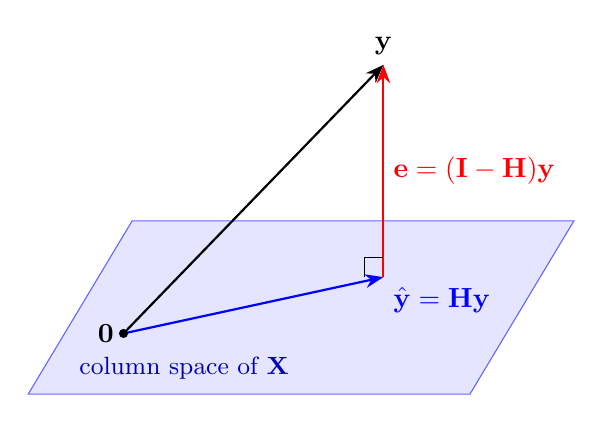
\begin{tikzpicture}[scale=1.1]
\filldraw[fill=blue!10,draw=blue!60] (-0.5,-0.6) -- (4.6,-0.6) -- (5.8,1.4) -- (0.7,1.4) -- cycle;
\node[blue!70!black] at (1.3,-0.3) {\small column space of $\mathbf{X}$};
\coordinate (O) at (0.6,0.1);
\coordinate (Y) at (3.6,3.2);
\coordinate (P) at (3.6,0.75);
\draw[-Stealth,thick] (O) -- (Y) node[above] {$\mathbf{y}$};
\draw[-Stealth,thick,blue] (O) -- (P) node[below right] {$\hat{\mathbf{y}} = \mathbf{Hy}$};
\draw[-Stealth,thick,red] (P) -- (Y) node[midway,right] {$\mathbf{e} = (\mathbf{I} - \mathbf{H})\mathbf{y}$};
\draw (3.6,0.98) -- (3.38,0.98) -- (3.38,0.75);
\fill (O) circle (1.5pt) node[left] {$\mathbf{0}$};
\end{tikzpicture}
\caption{Least squares as projection: $\hat{\mathbf{y}}$ is the foot of the perpendicular from
$\mathbf{y}$ to the column space of $\mathbf{X}$, and $\mathbf{e}$ is perpendicular to it.}
\label{fig:projection}
\end{figure}

\begin{exa}\label{exa:crop-resid}
Find the fitted values and residuals for the crop data and check
$\mathbf{X}^\top\mathbf{e} = \mathbf{0}$.
\end{exa}

\begin{solution}
From $\hat y = 3 + 2x_1 + x_2$:
\begin{center}
\begin{tabular}{c|cccccc}
Plot & 1 & 2 & 3 & 4 & 5 & 6 \\
\hline
$y_i$ & 6 & 9 & 11 & 10 & 15 & 18 \\
$\hat y_i$ & 7 & 8 & 10 & 11 & 15 & 18 \\
$e_i$ & $-1$ & $1$ & $1$ & $-1$ & $0$ & $0$ \\
\end{tabular}
\end{center}
The three rows of $\mathbf{X}^\top\mathbf{e}$ are
\begin{align*}
\textstyle\sum e_i &= -1 + 1 + 1 - 1 + 0 + 0 = 0, \\
\textstyle\sum x_{i1} e_i &= -1 + 2 + 2 - 3 + 0 + 0 = 0, \\
\textstyle\sum x_{i2} e_i &= -2 + 1 + 3 - 2 + 0 + 0 = 0 .
\end{align*}
The leverages $h_{ii} = \mathbf{x}_i^\top(\mathbf{X}^\top\mathbf{X})^{-1}\mathbf{x}_i$, where
$\mathbf{x}_i^\top$ is the $i$th row of $\mathbf{X}$, work out as
\[
0.421, \quad 0.587, \quad 0.397, \quad 0.230, \quad 0.587, \quad 0.778 .
\]
They lie between $0$ and $1$ and add up to $3 = p$, as Theorem~\ref{thm:hat} requires. Plot~6,
with by far the most fertiliser, has the largest leverage.
\end{solution}

\subsection{Properties of the least-squares estimator}
\begin{thm}\label{thm:beta-props}
Under A1--A3, $\hat{\boldsymbol\beta}$ is unbiased, with covariance matrix
\[
E(\hat{\boldsymbol\beta}) = \boldsymbol\beta, \qquad
\operatorname{Var}(\hat{\boldsymbol\beta}) = \sigma^2(\mathbf{X}^\top\mathbf{X})^{-1} = \sigma^2\mathbf{C} .
\]
So $\operatorname{Var}(\hat\beta_j) = \sigma^2 C_{jj}$ and
$\operatorname{Cov}(\hat\beta_i, \hat\beta_j) = \sigma^2 C_{ij}$, where the rows and columns of
$\mathbf{C}$ are numbered $0, 1, \dots, k$ to match the coefficients.
\end{thm}

\begin{proof}
$\hat{\boldsymbol\beta} = \mathbf{C}\mathbf{X}^\top\mathbf{y}$ is a linear function of
$\mathbf{y}$. By Lemma~\ref{lem:linear-rv},
$E(\hat{\boldsymbol\beta}) = \mathbf{C}\mathbf{X}^\top\mathbf{X}\boldsymbol\beta = \boldsymbol\beta$, and
\[
\operatorname{Var}(\hat{\boldsymbol\beta}) = \mathbf{C}\mathbf{X}^\top(\sigma^2\mathbf{I})\mathbf{X}\mathbf{C}^\top
= \sigma^2\mathbf{C}(\mathbf{X}^\top\mathbf{X})\mathbf{C} = \sigma^2\mathbf{C} . \qedhere
\]
\end{proof}

For simple regression, $\sigma^2\mathbf{C}$ is $\sigma^2/(nS_{xx})$ times the matrix in
Example~\ref{exa:slr-matrix}, and its entries are exactly the variances and covariance of
Theorems~\ref{thm:b1} and~\ref{thm:b0} (Problem~\ref{prob:slr-matrix}).

\begin{thm}[Gauss--Markov]\label{thm:gauss-markov-general}
Under A1--A3, let $\mathbf{c}$ be any constant vector. Among all estimators of
$\mathbf{c}^\top\boldsymbol\beta$ that are linear in $\mathbf{y}$ and unbiased,
$\mathbf{c}^\top\hat{\boldsymbol\beta}$ has the smallest variance. In particular each
$\hat\beta_j$ is the best linear unbiased estimator of $\beta_j$.
\end{thm}

\begin{proof}
Let $\mathbf{a}^\top\mathbf{y}$ be linear and unbiased for $\mathbf{c}^\top\boldsymbol\beta$:
$E(\mathbf{a}^\top\mathbf{y}) = \mathbf{a}^\top\mathbf{X}\boldsymbol\beta = \mathbf{c}^\top\boldsymbol\beta$
for every $\boldsymbol\beta$, which forces $\mathbf{X}^\top\mathbf{a} = \mathbf{c}$.
The least-squares estimator is $\mathbf{c}^\top\hat{\boldsymbol\beta} = \mathbf{a}_0^\top\mathbf{y}$
with $\mathbf{a}_0 = \mathbf{X}\mathbf{C}\mathbf{c}$. Let $\mathbf{d} = \mathbf{a} - \mathbf{a}_0$. Then
\[
\mathbf{X}^\top\mathbf{d} = \mathbf{c} - \mathbf{X}^\top\mathbf{X}\mathbf{C}\mathbf{c} = \mathbf{c} - \mathbf{c} = \mathbf{0},
\qquad\text{so}\qquad
\mathbf{a}_0^\top\mathbf{d} = \mathbf{c}^\top\mathbf{C}\mathbf{X}^\top\mathbf{d} = 0 .
\]
Since $\operatorname{Var}(\mathbf{y}) = \sigma^2\mathbf{I}$, Lemma~\ref{lem:linear-rv} gives
$\operatorname{Var}(\mathbf{a}^\top\mathbf{y}) = \sigma^2\mathbf{a}^\top\mathbf{a}$, and
\[
\mathbf{a}^\top\mathbf{a} = (\mathbf{a}_0 + \mathbf{d})^\top(\mathbf{a}_0 + \mathbf{d})
= \mathbf{a}_0^\top\mathbf{a}_0 + \mathbf{d}^\top\mathbf{d} \ge \mathbf{a}_0^\top\mathbf{a}_0 .
\]
So $\operatorname{Var}(\mathbf{a}^\top\mathbf{y}) \ge \operatorname{Var}(\mathbf{c}^\top\hat{\boldsymbol\beta})$,
with equality only when $\mathbf{d} = \mathbf{0}$. Taking $\mathbf{c}$ with a $1$ in place $j$
and zeros elsewhere gives the statement about $\hat\beta_j$.
\end{proof}

This also settles the claim made after Theorem~\ref{thm:gauss-markov}: in simple regression
$\hat\beta_0$, as well as $\hat\beta_1$, is best linear unbiased.

\subsection{Estimation of $\sigma^2$ in multiple regression}
\begin{thm}\label{thm:ssres-matrix}
\begin{enumerate}[label=(\roman*)]
\item $SS_{\mathrm{Res}} = \mathbf{e}^\top\mathbf{e} = \mathbf{y}^\top(\mathbf{I} - \mathbf{H})\mathbf{y}
= \mathbf{y}^\top\mathbf{y} - \hat{\boldsymbol\beta}^\top\mathbf{X}^\top\mathbf{y}$.
\item Under A1--A3, $E(SS_{\mathrm{Res}}) = (n - p)\sigma^2$, so
\[
\hat\sigma^2 = MS_{\mathrm{Res}} = \frac{SS_{\mathrm{Res}}}{n - p}
\]
is unbiased for $\sigma^2$.
\end{enumerate}
\end{thm}

\begin{proof}
(i) By Theorem~\ref{thm:hat}(i),
$\mathbf{e}^\top\mathbf{e} = \mathbf{y}^\top(\mathbf{I} - \mathbf{H})^\top(\mathbf{I} - \mathbf{H})\mathbf{y} = \mathbf{y}^\top(\mathbf{I} - \mathbf{H})\mathbf{y}$.
And $\mathbf{y}^\top\mathbf{H}\mathbf{y} = \mathbf{y}^\top\mathbf{X}\mathbf{C}\mathbf{X}^\top\mathbf{y} = \mathbf{y}^\top\mathbf{X}\hat{\boldsymbol\beta} = \hat{\boldsymbol\beta}^\top\mathbf{X}^\top\mathbf{y}$.

(ii) By Lemma~\ref{lem:quad-form} with $\mathbf{A} = \mathbf{I} - \mathbf{H}$,
$\boldsymbol\mu = \mathbf{X}\boldsymbol\beta$ and $\mathbf{V} = \sigma^2\mathbf{I}$,
\[
E(SS_{\mathrm{Res}}) = \sigma^2\operatorname{tr}(\mathbf{I} - \mathbf{H})
  + \boldsymbol\beta^\top\mathbf{X}^\top(\mathbf{I} - \mathbf{H})\mathbf{X}\boldsymbol\beta
= \sigma^2(n - p) + 0 ,
\]
by Theorem~\ref{thm:hat}(iv) and (ii).
\end{proof}

With $k = 1$, $p = 2$ and this is Theorem~\ref{thm:e-ssres}, proved now in two lines. One
degree of freedom is lost for each estimated coefficient. The \textbf{standard error} of
$\hat\beta_j$ is
\[
\operatorname{se}(\hat\beta_j) = \sqrt{\hat\sigma^2 C_{jj}} .
\]

\begin{exa}\label{exa:crop-sigma}
Estimate $\sigma^2$ for the crop data, and find the standard errors of the coefficients.
\end{exa}

\begin{solution}
From the residuals, $SS_{\mathrm{Res}} = 1 + 1 + 1 + 1 + 0 + 0 = 4$. Check with
Theorem~\ref{thm:ssres-matrix}(i): $\mathbf{y}^\top\mathbf{y} = \sum y_i^2 = 887$ and
\[
\hat{\boldsymbol\beta}^\top\mathbf{X}^\top\mathbf{y} = 3(69) + 2(244) + 1(188) = 207 + 488 + 188 = 883,
\]
so $SS_{\mathrm{Res}} = 887 - 883 = 4$. With $n - p = 6 - 3 = 3$,
\[
\hat\sigma^2 = \frac43 = 1.3333 .
\]
The diagonal of $\mathbf{C}$ is $C_{00} = 510/378$, $C_{11} = 33/378$, $C_{22} = 96/378$, so
\begin{align*}
\operatorname{se}(\hat\beta_0) &= \sqrt{1.3333 \times 510/378} = 1.341, \\
\operatorname{se}(\hat\beta_1) &= \sqrt{1.3333 \times 33/378} = 0.341, \\
\operatorname{se}(\hat\beta_2) &= \sqrt{1.3333 \times 96/378} = 0.582 .
\end{align*}
The estimated covariance of $\hat\beta_1$ and $\hat\beta_2$ is
$\hat\sigma^2 C_{12} = 1.3333 \times (-30/378) = -0.106$. It is negative because, in these
data, fertiliser and rainfall tend to rise together: credit for a high yield can be shifted
from one to the other, so an overestimate of one coefficient tends to go with an
underestimate of the other.
\end{solution}

\subsection{Distribution theory under normality}
From here on A4 is assumed: $\boldsymbol\varepsilon \sim N_n(\mathbf{0}, \sigma^2\mathbf{I})$.
The distributional facts (F1)--(F3) of Subsection~\ref{ssec:distributions} are used again,
together with one result from linear algebra, the \textbf{spectral theorem}: a symmetric
matrix $\mathbf{A}$ can be written $\mathbf{A} = \mathbf{P}\boldsymbol\Lambda\mathbf{P}^\top$,
where $\boldsymbol\Lambda$ is the diagonal matrix of its eigenvalues and $\mathbf{P}$ is
orthogonal, $\mathbf{P}^\top\mathbf{P} = \mathbf{I}$.

\begin{lem}\label{lem:idempotent-chisq}
Let $\mathbf{z} \sim N_n(\mathbf{0}, \sigma^2\mathbf{I})$ and let $\mathbf{A}$ be symmetric
and idempotent.
\begin{enumerate}[label=(\roman*)]
\item The eigenvalues of $\mathbf{A}$ are $0$ or $1$, and the number equal to $1$ is
$r = \operatorname{tr}(\mathbf{A})$, the rank of $\mathbf{A}$.
\item $\mathbf{z}^\top\mathbf{A}\mathbf{z}/\sigma^2 \sim \chi^2_r$.
\item If $\mathbf{B}$ is also symmetric and idempotent and $\mathbf{AB} = \mathbf{0}$, then
$\mathbf{z}^\top\mathbf{A}\mathbf{z}$ and $\mathbf{z}^\top\mathbf{B}\mathbf{z}$ are independent.
\end{enumerate}
\end{lem}

\begin{proof}
(i) If $\mathbf{Av} = \lambda\mathbf{v}$ with $\mathbf{v} \neq \mathbf{0}$, then
$\lambda\mathbf{v} = \mathbf{Av} = \mathbf{A}^2\mathbf{v} = \lambda^2\mathbf{v}$, so
$\lambda^2 = \lambda$ and $\lambda$ is $0$ or $1$. The trace of
$\mathbf{P}\boldsymbol\Lambda\mathbf{P}^\top$ is
$\operatorname{tr}(\boldsymbol\Lambda\mathbf{P}^\top\mathbf{P}) = \operatorname{tr}(\boldsymbol\Lambda)$
by Lemma~\ref{lem:trace}, the sum of the eigenvalues, which here is the number of ones.

(ii) Let $\mathbf{w} = \mathbf{P}^\top\mathbf{z}/\sigma$. By Lemma~\ref{lem:linear-rv} it is
normal with mean $\mathbf{0}$ and covariance
$\mathbf{P}^\top(\sigma^2\mathbf{I})\mathbf{P}/\sigma^2 = \mathbf{I}$, so its entries are
independent $N(0,1)$. Then
\[
\frac{\mathbf{z}^\top\mathbf{A}\mathbf{z}}{\sigma^2}
= \mathbf{w}^\top\mathbf{P}^\top\mathbf{A}\mathbf{P}\mathbf{w} = \mathbf{w}^\top\boldsymbol\Lambda\mathbf{w}
= \sum_{i\colon \lambda_i = 1} w_i^2 ,
\]
a sum of $r$ squared independent standard normals, which is $\chi^2_r$ by (F2).

(iii) $\mathbf{Az}$ and $\mathbf{Bz}$ are jointly normal, with
$\operatorname{Cov}(\mathbf{Az}, \mathbf{Bz}) = \mathbf{A}(\sigma^2\mathbf{I})\mathbf{B}^\top = \sigma^2\mathbf{AB} = \mathbf{0}$,
so they are independent by (F1). And
$\mathbf{z}^\top\mathbf{A}\mathbf{z} = \mathbf{z}^\top\mathbf{A}^\top\mathbf{A}\mathbf{z} = (\mathbf{Az})^\top(\mathbf{Az})$
is a function of $\mathbf{Az}$ alone; likewise $\mathbf{z}^\top\mathbf{B}\mathbf{z}$ of $\mathbf{Bz}$.
\end{proof}

\begin{thm}\label{thm:mlr-dist}
Under A1--A4,
\begin{enumerate}[label=(\roman*)]
\item $\hat{\boldsymbol\beta} \sim N_p\bigl(\boldsymbol\beta, \sigma^2\mathbf{C}\bigr)$, so each $\hat\beta_j \sim N(\beta_j, \sigma^2 C_{jj})$;
\item $SS_{\mathrm{Res}}/\sigma^2 \sim \chi^2_{n-p}$;
\item $SS_{\mathrm{Res}}$ is independent of $\hat{\boldsymbol\beta}$.
\end{enumerate}
\end{thm}

\begin{proof}
(i) $\hat{\boldsymbol\beta}$ is linear in $\mathbf{y}$, hence normal by (F1), with the mean
and covariance of Theorem~\ref{thm:beta-props}.

(ii) $(\mathbf{I} - \mathbf{H})\mathbf{y} = (\mathbf{I} - \mathbf{H})\boldsymbol\varepsilon$
because $(\mathbf{I} - \mathbf{H})\mathbf{X} = \mathbf{0}$, so
$SS_{\mathrm{Res}} = \boldsymbol\varepsilon^\top(\mathbf{I} - \mathbf{H})\boldsymbol\varepsilon$.
$\mathbf{I} - \mathbf{H}$ is symmetric and idempotent with trace $n - p$
(Theorem~\ref{thm:hat}), so Lemma~\ref{lem:idempotent-chisq}(ii) applies.

(iii) $\hat{\boldsymbol\beta} - \boldsymbol\beta = \mathbf{C}\mathbf{X}^\top\boldsymbol\varepsilon$
and $\mathbf{e} = (\mathbf{I} - \mathbf{H})\boldsymbol\varepsilon$ are jointly normal, with
\[
\operatorname{Cov}\bigl(\mathbf{C}\mathbf{X}^\top\boldsymbol\varepsilon,\ (\mathbf{I} - \mathbf{H})\boldsymbol\varepsilon\bigr)
= \sigma^2\mathbf{C}\bigl((\mathbf{I} - \mathbf{H})\mathbf{X}\bigr)^\top = \mathbf{0} .
\]
So $\hat{\boldsymbol\beta}$ is independent of $\mathbf{e}$, and hence of
$SS_{\mathrm{Res}} = \mathbf{e}^\top\mathbf{e}$.
\end{proof}

\subsection{Test for significance of regression}
The first question about a fitted model is whether it is of any use at all: is there a
linear relationship between $y$ and \emph{any} of the regressors? The hypotheses are
\[
H_0\colon \beta_1 = \beta_2 = \cdots = \beta_k = 0
\qquad\text{against}\qquad
H_1\colon \beta_j \neq 0 \text{ for at least one } j .
\]
The intercept is not included: $H_0$ says that $E(y) = \beta_0$ whatever the regressors are.

As in simple regression, the total sum of squares splits as
$SS_T = SS_R + SS_{\mathrm{Res}}$ (Problem~\ref{prob:anova-matrix}), where
\begin{align*}
SS_T &= \mathbf{y}^\top\mathbf{y} - \frac{\left(\sum y_i\right)^2}{n}, \\
SS_R &= \hat{\boldsymbol\beta}^\top\mathbf{X}^\top\mathbf{y} - \frac{\left(\sum y_i\right)^2}{n}, \\
SS_{\mathrm{Res}} &= \mathbf{y}^\top\mathbf{y} - \hat{\boldsymbol\beta}^\top\mathbf{X}^\top\mathbf{y} .
\end{align*}
$SS_R$ has $k$ degrees of freedom, one for each slope, and $SS_{\mathrm{Res}}$ has $n - p$.

\begin{thm}\label{thm:overall-F}
Under A1--A4, when $H_0\colon \beta_1 = \cdots = \beta_k = 0$ is true,
\[
F_0 = \frac{SS_R/k}{SS_{\mathrm{Res}}/(n-p)} = \frac{MS_R}{MS_{\mathrm{Res}}} \sim F_{k, n-p} .
\]
When $H_0$ is false, $E(SS_R) > k\sigma^2$, so large values of $F_0$ are evidence against $H_0$.
\end{thm}

\begin{proof}
Let $\mathbf{1}$ be the vector of ones and $\bar{\mathbf{J}} = \frac1n\mathbf{1}\mathbf{1}^\top$,
the $n \times n$ matrix with every entry $1/n$. Then $\mathbf{y}^\top\bar{\mathbf{J}}\mathbf{y} = \left(\sum y_i\right)^2/n$,
and $\mathbf{y}^\top\mathbf{H}\mathbf{y} = \hat{\boldsymbol\beta}^\top\mathbf{X}^\top\mathbf{y}$
(proof of Theorem~\ref{thm:ssres-matrix}), so
$SS_R = \mathbf{y}^\top(\mathbf{H} - \bar{\mathbf{J}})\mathbf{y}$.

\emph{Properties of $\mathbf{H} - \bar{\mathbf{J}}$.} $\mathbf{1}$ is the first column of
$\mathbf{X}$, so $\mathbf{H}\mathbf{1} = \mathbf{1}$ by Theorem~\ref{thm:hat}(ii). Hence
$\mathbf{H}\bar{\mathbf{J}} = \bar{\mathbf{J}}$, and transposing, $\bar{\mathbf{J}}\mathbf{H} = \bar{\mathbf{J}}$.
Also $\bar{\mathbf{J}}^2 = \frac{1}{n^2}\mathbf{1}(\mathbf{1}^\top\mathbf{1})\mathbf{1}^\top = \bar{\mathbf{J}}$. So
\begin{align*}
(\mathbf{H} - \bar{\mathbf{J}})^2 &= \mathbf{H} - \bar{\mathbf{J}} - \bar{\mathbf{J}} + \bar{\mathbf{J}} = \mathbf{H} - \bar{\mathbf{J}}, \\
(\mathbf{H} - \bar{\mathbf{J}})(\mathbf{I} - \mathbf{H}) &= \mathbf{H} - \mathbf{H} - \bar{\mathbf{J}} + \bar{\mathbf{J}} = \mathbf{0},
\end{align*}
and $\operatorname{tr}(\mathbf{H} - \bar{\mathbf{J}}) = p - 1 = k$. It is symmetric and
idempotent of rank $k$.

\emph{Under $H_0$}, $\mathbf{X}\boldsymbol\beta = \beta_0\mathbf{1}$, and
$(\mathbf{H} - \bar{\mathbf{J}})\mathbf{1} = \mathbf{1} - \mathbf{1} = \mathbf{0}$. So
$(\mathbf{H} - \bar{\mathbf{J}})\mathbf{y} = (\mathbf{H} - \bar{\mathbf{J}})\boldsymbol\varepsilon$ and
$SS_R = \boldsymbol\varepsilon^\top(\mathbf{H} - \bar{\mathbf{J}})\boldsymbol\varepsilon$. Since also
$SS_{\mathrm{Res}} = \boldsymbol\varepsilon^\top(\mathbf{I} - \mathbf{H})\boldsymbol\varepsilon$,
Lemma~\ref{lem:idempotent-chisq} gives $SS_R/\sigma^2 \sim \chi^2_k$ and
$SS_{\mathrm{Res}}/\sigma^2 \sim \chi^2_{n-p}$, independently, and (F3) gives the $F$ distribution.

\emph{When $H_0$ is false.} By Lemma~\ref{lem:quad-form},
$E(SS_R) = \sigma^2\operatorname{tr}(\mathbf{H} - \bar{\mathbf{J}}) + \boldsymbol\mu^\top(\mathbf{H} - \bar{\mathbf{J}})\boldsymbol\mu$
with $\boldsymbol\mu = \mathbf{X}\boldsymbol\beta$. Since $\mathbf{H}\boldsymbol\mu = \boldsymbol\mu$,
the second term is $\boldsymbol\mu^\top(\mathbf{I} - \bar{\mathbf{J}})\boldsymbol\mu = \sum (\mu_i - \bar\mu)^2$,
which is positive unless all the $\mu_i$ are equal. With $\mathbf{X}$ of full rank that happens
only when $\beta_1 = \cdots = \beta_k = 0$.
\end{proof}

Reject $H_0$ at level $\alpha$ when $F_0 > F_{\alpha, k, n-p}$. The working goes in an
ANOVA table:
\begin{center}
\begin{tabular}{lcccc}
\hline
Source & Sum of squares & df & Mean square & $F_0$ \\
\hline
Regression & $SS_R$ & $k$ & $MS_R = SS_R/k$ & $MS_R/MS_{\mathrm{Res}}$ \\
Residual & $SS_{\mathrm{Res}}$ & $n - p$ & $MS_{\mathrm{Res}}$ & \\
\hline
Total & $SS_T$ & $n - 1$ & & \\
\hline
\end{tabular}
\end{center}
With $k = 1$ this is exactly the table of Subsection~\ref{ssec:anova}.

\begin{exa}\label{exa:crop-anova}
Test significance of regression for the crop data at the 5\% level.
\end{exa}

\begin{solution}
From Examples~\ref{exa:crop-fit} and~\ref{exa:crop-sigma}: $\sum y_i = 69$,
$\mathbf{y}^\top\mathbf{y} = 887$ and $\hat{\boldsymbol\beta}^\top\mathbf{X}^\top\mathbf{y} = 883$.
The correction term is $69^2/6 = 793.5$, so
\begin{align*}
SS_T &= 887 - 793.5 = 93.5, \\
SS_R &= 883 - 793.5 = 89.5, \\
SS_{\mathrm{Res}} &= 887 - 883 = 4 .
\end{align*}
\begin{center}
\begin{tabular}{lcccc}
\hline
Source & SS & df & MS & $F_0$ \\
\hline
Regression & 89.5 & 2 & 44.75 & 33.56 \\
Residual & 4.0 & 3 & 1.3333 & \\
\hline
Total & 93.5 & 5 & & \\
\hline
\end{tabular}
\end{center}
$F_{0.05,2,3} = 9.55$, and $33.56 > 9.55$, so reject $H_0\colon \beta_1 = \beta_2 = 0$
($p = 0.009$). Yield is linearly related to at least one of fertiliser and rainfall.
\end{solution}

\subsection{$R^2$ and adjusted $R^2$}
The coefficient of determination is defined as before, $R^2 = SS_R/SS_T = 1 - SS_{\mathrm{Res}}/SS_T$.
For the crop data, $R^2 = 89.5/93.5 = 0.957$.

\begin{thm}\label{thm:r2-increase}
Adding a regressor to a model never decreases $R^2$.
\end{thm}

\begin{proof}
$SS_T$ does not depend on the model. The larger model can reproduce any fit of the smaller
one by setting the new coefficient to zero, so its minimum of $S(\boldsymbol\beta)$, which
is its $SS_{\mathrm{Res}}$, is no greater. So $1 - SS_{\mathrm{Res}}/SS_T$ cannot fall.
\end{proof}

So $R^2$ always favours the bigger model, even when the added regressor is pure noise. To
compare models with different numbers of parameters, $R^2$ is adjusted by replacing each sum
of squares with its mean square:
\[
R^2_{\mathrm{adj}} = 1 - \frac{SS_{\mathrm{Res}}/(n - p)}{SS_T/(n - 1)} .
\]
An extra regressor lowers $SS_{\mathrm{Res}}$ but also lowers $n - p$, so $R^2_{\mathrm{adj}}$
rises only if the regressor earns its degree of freedom. For the crop data,
\[
R^2_{\mathrm{adj}} = 1 - \frac{4/3}{93.5/5} = 1 - \frac{1.3333}{18.7} = 0.929 .
\]

\subsection{Tests on individual coefficients}
\begin{thm}\label{thm:t-mlr}
Under A1--A4,
\[
\frac{\hat\beta_j - \beta_j}{\operatorname{se}(\hat\beta_j)} \sim t_{n-p},
\qquad \operatorname{se}(\hat\beta_j) = \sqrt{\hat\sigma^2 C_{jj}} .
\]
\end{thm}

\begin{proof}
$(\hat\beta_j - \beta_j)/\sqrt{\sigma^2 C_{jj}} \sim N(0,1)$ and
$(n-p)\hat\sigma^2/\sigma^2 \sim \chi^2_{n-p}$, independently, by Theorem~\ref{thm:mlr-dist}.
By (F3) their ratio, $Z/\sqrt{V/(n-p)}$, is $t_{n-p}$, and $\sigma$ cancels as in
Theorem~\ref{thm:t-slope}.
\end{proof}

To test $H_0\colon \beta_j = 0$, use $t_0 = \hat\beta_j/\operatorname{se}(\hat\beta_j)$ and
reject when $|t_0| > t_{\alpha/2, n-p}$.

\begin{remark}
This is a \textbf{marginal} or \textbf{partial} test: it asks whether $x_j$ adds anything
\emph{given that all the other regressors are in the model}. Its verdict can change when other
regressors are added or removed.
\end{remark}

\begin{exa}\label{exa:crop-t}
Test the significance of each regressor in the crop model at the 5\% level.
\end{exa}

\begin{solution}
With $t_{0.025,3} = 3.182$ and the standard errors of Example~\ref{exa:crop-sigma}:
\begin{center}
\begin{tabular}{lcccc}
\hline
Coefficient & Estimate & se & $t_0$ & Decision \\
\hline
$\beta_1$ (fertiliser) & 2 & 0.3412 & 5.862 & reject $H_0$ ($p = 0.010$) \\
$\beta_2$ (rainfall) & 1 & 0.5819 & 1.719 & do not reject ($p = 0.184$) \\
\hline
\end{tabular}
\end{center}
Fertiliser is significant. Once fertiliser is in the model, rainfall does not add a
significant amount; that is not the same as saying rainfall does not affect yield.
\end{solution}

\subsection{The extra-sum-of-squares principle}\label{ssec:extra-ss}
The overall $F$-test asks about all the slopes; the $t$-test asks about one. Often the
question is about a \emph{group} of coefficients: for instance, whether two weather variables
together add anything to a model that already contains the fertiliser and soil variables.

Split the coefficients as $\boldsymbol\beta = (\boldsymbol\beta_1^\top, \boldsymbol\beta_2^\top)^\top$,
where $\boldsymbol\beta_2$ holds the $r$ coefficients being tested, and split
$\mathbf{X} = [\mathbf{X}_1 \ \mathbf{X}_2]$ to match, so that
$\mathbf{X}\boldsymbol\beta = \mathbf{X}_1\boldsymbol\beta_1 + \mathbf{X}_2\boldsymbol\beta_2$.
We test $H_0\colon \boldsymbol\beta_2 = \mathbf{0}$.

\begin{defn}
Let $SS_R(\boldsymbol\beta)$ be the regression sum of squares of the full model and
$SS_R(\boldsymbol\beta_1)$ that of the \textbf{reduced model} $\mathbf{y} = \mathbf{X}_1\boldsymbol\beta_1 + \boldsymbol\varepsilon$.
The \textbf{extra sum of squares} due to $\boldsymbol\beta_2$, given $\boldsymbol\beta_1$, is
\[
SS_R(\boldsymbol\beta_2 \mid \boldsymbol\beta_1) = SS_R(\boldsymbol\beta) - SS_R(\boldsymbol\beta_1),
\]
the increase in the regression sum of squares, or equivalently the decrease in $SS_{\mathrm{Res}}$,
from adding $\mathbf{X}_2$ to the model.
\end{defn}

\begin{thm}[Partial $F$-test]\label{thm:partial-F}
Under A1--A4, when $H_0\colon \boldsymbol\beta_2 = \mathbf{0}$ is true,
\[
F_0 = \frac{SS_R(\boldsymbol\beta_2 \mid \boldsymbol\beta_1)/r}{MS_{\mathrm{Res}}} \sim F_{r, n-p},
\]
where $MS_{\mathrm{Res}}$ is from the full model.
\end{thm}

\begin{proof}
Let $\mathbf{H}_1 = \mathbf{X}_1(\mathbf{X}_1^\top\mathbf{X}_1)^{-1}\mathbf{X}_1^\top$ be the
hat matrix of the reduced model. The correction term $\left(\sum y_i\right)^2/n$ is the same in
both regression sums of squares and cancels, so
$SS_R(\boldsymbol\beta_2 \mid \boldsymbol\beta_1) = \mathbf{y}^\top(\mathbf{H} - \mathbf{H}_1)\mathbf{y}$.

The columns of $\mathbf{X}_1$ are columns of $\mathbf{X}$, so $\mathbf{H}\mathbf{X}_1 = \mathbf{X}_1$
by Theorem~\ref{thm:hat}(ii), hence $\mathbf{H}\mathbf{H}_1 = \mathbf{H}_1$ and, transposing,
$\mathbf{H}_1\mathbf{H} = \mathbf{H}_1$. Exactly as for $\mathbf{H} - \bar{\mathbf{J}}$ in
Theorem~\ref{thm:overall-F}, it follows that $\mathbf{H} - \mathbf{H}_1$ is symmetric and
idempotent, that $(\mathbf{H} - \mathbf{H}_1)(\mathbf{I} - \mathbf{H}) = \mathbf{0}$, and that
its rank is $\operatorname{tr}(\mathbf{H}) - \operatorname{tr}(\mathbf{H}_1) = p - (p - r) = r$.

Under $H_0$, $\mathbf{X}\boldsymbol\beta = \mathbf{X}_1\boldsymbol\beta_1$, and
$(\mathbf{H} - \mathbf{H}_1)\mathbf{X}_1 = \mathbf{X}_1 - \mathbf{X}_1 = \mathbf{0}$. So
$SS_R(\boldsymbol\beta_2 \mid \boldsymbol\beta_1) = \boldsymbol\varepsilon^\top(\mathbf{H} - \mathbf{H}_1)\boldsymbol\varepsilon$,
and Lemma~\ref{lem:idempotent-chisq} and (F3) finish the proof as before.
\end{proof}

The overall test of Theorem~\ref{thm:overall-F} is the case where $\mathbf{X}_1 = \mathbf{1}$,
so that $\mathbf{H}_1 = \bar{\mathbf{J}}$.

\begin{exa}\label{exa:crop-partial}
For the crop data, use the extra-sum-of-squares principle to test whether rainfall adds to a
model that already contains fertiliser.
\end{exa}

\begin{solution}
\emph{Reduced model:} $y = \beta_0 + \beta_1 x_1 + \varepsilon$, a simple regression. From the
table of Example~\ref{exa:crop-fit},
\[
S_{x_1x_1} = 70 - \frac{18^2}{6} = 16, \qquad S_{x_1y} = 244 - \frac{18 \times 69}{6} = 37,
\]
so $SS_R(\beta_1) = S_{x_1y}^2/S_{x_1x_1} = 37^2/16 = 85.5625$.

\emph{Extra sum of squares:}
$SS_R(\beta_2 \mid \beta_1) = 89.5 - 85.5625 = 3.9375$, on $r = 1$ degree of freedom.

\emph{Test:}
\[
F_0 = \frac{3.9375/1}{1.3333} = 2.953 < F_{0.05,1,3} = 10.13 ,
\]
so do not reject $H_0\colon \beta_2 = 0$. This agrees with the $t$-test of
Example~\ref{exa:crop-t}, and $t_0^2 = 1.7185^2 = 2.953 = F_0$: when $r = 1$, the partial
$F$-test and the $t$-test are the same test (Theorem~\ref{thm:added-variable}).

The order in which regressors are added matters. Fitting rainfall alone gives
$SS_R(\beta_2) = 43.68$, so $SS_R(\beta_1 \mid \beta_2) = 89.5 - 43.68 = 45.82$: fertiliser
added to rainfall explains far more than rainfall added to fertiliser.
\end{solution}

The next result explains why a partial $F$-test on one coefficient is the same as its
$t$-test, and gives a picture of what a single coefficient in a multiple regression measures.

\begin{thm}[Added-variable, or Frisch--Waugh, theorem]\label{thm:added-variable}
Let $\mathbf{x}$ be the column of $\mathbf{X}$ belonging to $\beta_j$, and let $\mathbf{X}_1$
hold the other columns, with hat matrix $\mathbf{H}_1$. Let
$\mathbf{u} = (\mathbf{I} - \mathbf{H}_1)\mathbf{x}$, the residuals from regressing $x_j$ on
the other regressors. Then
\[
\hat\beta_j = \frac{\mathbf{u}^\top\mathbf{y}}{\mathbf{u}^\top\mathbf{u}}, \qquad
C_{jj} = \frac{1}{\mathbf{u}^\top\mathbf{u}}, \qquad
SS_R(\beta_j \mid \text{others}) = \frac{(\mathbf{u}^\top\mathbf{y})^2}{\mathbf{u}^\top\mathbf{u}} = \frac{\hat\beta_j^2}{C_{jj}} .
\]
Consequently the partial $F$ statistic for $\beta_j$ equals $t_0^2$.
\end{thm}

\begin{proof}
$\mathbf{u} \neq \mathbf{0}$, since $\mathbf{x}$ is not a combination of the columns of
$\mathbf{X}_1$ (full rank), and $\mathbf{X}_1^\top\mathbf{u} = \mathbf{0}$ by
Theorem~\ref{thm:hat}(iii) applied to the regression of $\mathbf{x}$ on $\mathbf{X}_1$; also
$\mathbf{H}_1\mathbf{u} = \mathbf{0}$. Put
\[
\mathbf{P} = \mathbf{H}_1 + \frac{\mathbf{u}\mathbf{u}^\top}{\mathbf{u}^\top\mathbf{u}} .
\]
We show that $\mathbf{Py}$ is the least-squares fit $\hat{\mathbf{y}}$. First, $\mathbf{Py}$
lies in the column space of $\mathbf{X}$, since $\mathbf{H}_1\mathbf{y}$ is a combination of
the columns of $\mathbf{X}_1$ and $\mathbf{u} = \mathbf{x} - \mathbf{H}_1\mathbf{x}$ is a
combination of $\mathbf{x}$ and those columns. Second, $\mathbf{y} - \mathbf{Py}$ is
perpendicular to every column of $\mathbf{X}$:
\begin{align*}
\mathbf{X}_1^\top(\mathbf{y} - \mathbf{Py}) &= \mathbf{X}_1^\top\mathbf{y} - \mathbf{X}_1^\top\mathbf{y} - \mathbf{0} = \mathbf{0}, \\
\mathbf{u}^\top(\mathbf{y} - \mathbf{Py}) &= \mathbf{u}^\top\mathbf{y} - 0 - \mathbf{u}^\top\mathbf{y} = 0 ,
\end{align*}
using $\mathbf{X}_1^\top\mathbf{H}_1 = \mathbf{X}_1^\top$, $\mathbf{X}_1^\top\mathbf{u} = \mathbf{0}$
and $\mathbf{u}^\top\mathbf{H}_1 = \mathbf{0}^\top$; and $\mathbf{x} = \mathbf{H}_1\mathbf{x} + \mathbf{u}$
is a combination of these. So $\mathbf{Py}$ satisfies the normal equations, and since the
least-squares fit is unique, $\hat{\mathbf{y}} = \mathbf{Py}$.

Now compare two ways of writing $\hat{\mathbf{y}}$. On one hand
$\hat{\mathbf{y}} = \mathbf{X}_1\hat{\boldsymbol\beta}_1 + \mathbf{x}\hat\beta_j
= (\mathbf{X}_1\hat{\boldsymbol\beta}_1 + \mathbf{H}_1\mathbf{x}\hat\beta_j) + \mathbf{u}\hat\beta_j$;
on the other, $\hat{\mathbf{y}} = \mathbf{H}_1\mathbf{y} + \mathbf{u}(\mathbf{u}^\top\mathbf{y})/(\mathbf{u}^\top\mathbf{u})$.
In each, the bracketed part lies in the column space of $\mathbf{X}_1$, which is perpendicular to
$\mathbf{u}$. Taking the inner product of both with $\mathbf{u}$ gives
$\mathbf{u}^\top\mathbf{u}\,\hat\beta_j = \mathbf{u}^\top\mathbf{y}$, the first formula.

It is linear in $\mathbf{y}$, so
$\operatorname{Var}(\hat\beta_j) = \sigma^2\mathbf{u}^\top\mathbf{u}/(\mathbf{u}^\top\mathbf{u})^2 = \sigma^2/\mathbf{u}^\top\mathbf{u}$,
and comparing with $\sigma^2 C_{jj}$ gives the second. Finally
$\mathbf{H} = \mathbf{P}$ (both give the fit of every $\mathbf{y}$), so
$\mathbf{H} - \mathbf{H}_1 = \mathbf{u}\mathbf{u}^\top/\mathbf{u}^\top\mathbf{u}$ and
$SS_R(\beta_j \mid \text{others}) = \mathbf{y}^\top(\mathbf{H} - \mathbf{H}_1)\mathbf{y} = (\mathbf{u}^\top\mathbf{y})^2/\mathbf{u}^\top\mathbf{u}$.
Dividing by $MS_{\mathrm{Res}}$,
\[
F_0 = \frac{\hat\beta_j^2/C_{jj}}{\hat\sigma^2} = \left( \frac{\hat\beta_j}{\sqrt{\hat\sigma^2 C_{jj}}} \right)^2 = t_0^2 . \qedhere
\]
\end{proof}

So $\hat\beta_j$ is the slope of a simple regression of $y$ on $\mathbf{u}$, the part of $x_j$
that the other regressors cannot explain. Only that part carries information about $\beta_j$.
When $x_j$ is nearly a combination of the other regressors, $\mathbf{u}$ is small,
$C_{jj} = 1/\mathbf{u}^\top\mathbf{u}$ is large, and $\hat\beta_j$ is imprecise. This is the
problem of \emph{multicollinearity}, which has a section of its own. For the crop data,
$C_{22} = 96/378$, and indeed $\hat\beta_2^2/C_{22} = 1 \times 378/96 = 3.9375$, the extra sum of
squares found in Example~\ref{exa:crop-partial}.

\subsection{Confidence and prediction intervals}
\begin{thm}\label{thm:mlr-intervals}
Under A1--A4, $100(1 - \alpha)\%$ intervals are:
\begin{enumerate}[label=(\roman*)]
\item for a coefficient $\beta_j$: $\hat\beta_j \pm t_{\alpha/2, n-p}\sqrt{\hat\sigma^2 C_{jj}}$;
\item for the mean response at $\mathbf{x}_0 = (1, x_{01}, \dots, x_{0k})^\top$:
\[
\hat y_0 \pm t_{\alpha/2, n-p}\sqrt{\hat\sigma^2\, \mathbf{x}_0^\top\mathbf{C}\mathbf{x}_0},
\qquad \hat y_0 = \mathbf{x}_0^\top\hat{\boldsymbol\beta} ;
\]
\item for a new observation at $\mathbf{x}_0$:
\[
\hat y_0 \pm t_{\alpha/2, n-p}\sqrt{\hat\sigma^2 \left(1 + \mathbf{x}_0^\top\mathbf{C}\mathbf{x}_0\right)} .
\]
\end{enumerate}
\end{thm}

\begin{proof}
(i) follows from Theorem~\ref{thm:t-mlr} exactly as in simple regression.

(ii) $\hat y_0 = \mathbf{x}_0^\top\hat{\boldsymbol\beta}$ is normal with mean
$\mathbf{x}_0^\top\boldsymbol\beta = E(y \mid \mathbf{x}_0)$ and, by Lemma~\ref{lem:linear-rv},
variance $\mathbf{x}_0^\top(\sigma^2\mathbf{C})\mathbf{x}_0$. It is a function of
$\hat{\boldsymbol\beta}$, so is independent of $SS_{\mathrm{Res}}$, and the $t$ argument applies.

(iii) A new observation $y_0 = \mathbf{x}_0^\top\boldsymbol\beta + \varepsilon_0$ is independent
of the sample, so $y_0 - \hat y_0$ has mean $0$ and variance
$\sigma^2 + \sigma^2\mathbf{x}_0^\top\mathbf{C}\mathbf{x}_0$, and the $t$ argument applies again.
\end{proof}

With $k = 1$, $\mathbf{x}_0^\top\mathbf{C}\mathbf{x}_0 = \frac1n + \frac{(x_0 - \bar x)^2}{S_{xx}}$,
recovering Theorems~\ref{thm:mean-response} and~\ref{thm:prediction}. Note that
$\mathbf{x}_0^\top\mathbf{C}\mathbf{x}_0$ is the leverage that the point $\mathbf{x}_0$ would
have if it were added to the data.

\begin{exa}\label{exa:crop-intervals}
For the crop data, find 95\% confidence intervals for $\beta_1$ and $\beta_2$. Then, for a plot
with $300$\,kg of fertiliser per hectare and $300$\,mm of rain, find a 95\% confidence interval
for the mean yield and a 95\% prediction interval for the yield of a single plot.
\end{exa}

\begin{solution}
With $t_{0.025,3} = 3.182$:
\begin{align*}
\beta_1&\colon\ 2 \pm 3.182 \times 0.3412 = 2 \pm 1.086, \quad\text{that is, } (0.914,\ 3.086); \\
\beta_2&\colon\ 1 \pm 3.182 \times 0.5819 = 1 \pm 1.852, \quad\text{that is, } (-0.852,\ 2.852).
\end{align*}
The interval for $\beta_2$ contains $0$, matching the $t$-test.

For the new plot, $\mathbf{x}_0 = (1, 3, 3)^\top$ and $\hat y_0 = 3 + 2(3) + 3 = 12$. Next,
\[
\mathbf{C}\mathbf{x}_0 = \frac{1}{378}\begin{bmatrix} 510 - 72 - 450 \\ -24 + 99 - 90 \\ -150 - 90 + 288 \end{bmatrix}
= \frac{1}{378}\begin{bmatrix} -12 \\ -15 \\ 48 \end{bmatrix},
\]
so
\[
\mathbf{x}_0^\top\mathbf{C}\mathbf{x}_0 = \frac{1}{378}\bigl(-12 + 3(-15) + 3(48)\bigr) = \frac{87}{378} = 0.2302 .
\]
\begin{itemize}
\item Mean yield: $12 \pm 3.182\sqrt{1.3333 \times 0.2302} = 12 \pm 3.182 \times 0.5540 = 12 \pm 1.763$,
that is, $(10.24,\ 13.76)$ tonnes per hectare.
\item A single plot: $12 \pm 3.182\sqrt{1.3333 \times 1.2302} = 12 \pm 3.182 \times 1.2807 = 12 \pm 4.076$,
that is, $(7.92,\ 16.08)$ tonnes per hectare.
\end{itemize}
\end{solution}

\begin{remark}[Hidden extrapolation]
With several regressors it is easy to extrapolate without noticing. A point can lie inside the
range of each regressor separately and still be far from the data jointly: here, a plot with
$x_1 = 6$ and $x_2 = 1$ is within both ranges, but no plot combined so much fertiliser with so
little rain, and indeed $\mathbf{x}_0^\top\mathbf{C}\mathbf{x}_0 = 846/378 = 2.24$ there.
A useful check is to compare $\mathbf{x}_0^\top\mathbf{C}\mathbf{x}_0$ with the
largest leverage in the data, $h_{\max}$; if it is larger, the prediction is an extrapolation.
For $\mathbf{x}_0 = (1, 3, 3)^\top$, $0.2302 < h_{\max} = 0.778$, so the intervals above are
safe.
\end{remark}

\subsection{Practice problems}
\begin{problem}\label{prob:orth}
A $2^2$ experiment with two centre points gave
\begin{center}
\begin{tabular}{c|cccccc}
$x_1$ & $-1$ & $1$ & $-1$ & $1$ & $0$ & $0$ \\
$x_2$ & $-1$ & $-1$ & $1$ & $1$ & $0$ & $0$ \\
\hline
$y$ & 20 & 30 & 26 & 38 & 29 & 31 \\
\end{tabular}
\end{center}
\begin{enumerate}[label=(\alph*)]
\item Form $\mathbf{X}^\top\mathbf{X}$ and $\mathbf{X}^\top\mathbf{y}$, and fit
$y = \beta_0 + \beta_1 x_1 + \beta_2 x_2 + \varepsilon$.
\item Find the residuals, $\hat\sigma^2$ and the standard errors.
\item Show that the three estimates are uncorrelated. What feature of the design causes this?
\end{enumerate}
\end{problem}

\begin{solution}
(a) $\sum x_{i1} = \sum x_{i2} = \sum x_{i1}x_{i2} = 0$ and $\sum x_{i1}^2 = \sum x_{i2}^2 = 4$, so
\[
\mathbf{X}^\top\mathbf{X} = \begin{bmatrix} 6 & 0 & 0 \\ 0 & 4 & 0 \\ 0 & 0 & 4 \end{bmatrix},
\qquad
\mathbf{X}^\top\mathbf{y} = \begin{bmatrix} 174 \\ 22 \\ 14 \end{bmatrix} .
\]
Here $\sum x_{i1}y_i = -20 + 30 - 26 + 38 = 22$ and $\sum x_{i2}y_i = -20 - 30 + 26 + 38 = 14$.
A diagonal matrix is inverted by inverting its diagonal, so
\[
\hat{\boldsymbol\beta} = \begin{bmatrix} 174/6 \\ 22/4 \\ 14/4 \end{bmatrix} = \begin{bmatrix} 29 \\ 5.5 \\ 3.5 \end{bmatrix},
\qquad \hat y = 29 + 5.5x_1 + 3.5x_2 .
\]
(b) The fitted values are $20, 31, 27, 38, 29, 29$, and the residuals $0, -1, -1, 0, 0, 2$.
$SS_{\mathrm{Res}} = 0 + 1 + 1 + 0 + 0 + 4 = 6$ (check: $\mathbf{y}^\top\mathbf{y} - \hat{\boldsymbol\beta}^\top\mathbf{X}^\top\mathbf{y} = 5222 - 5216 = 6$),
so $\hat\sigma^2 = 6/3 = 2$. Then $\operatorname{se}(\hat\beta_0) = \sqrt{2/6} = 0.577$ and
$\operatorname{se}(\hat\beta_1) = \operatorname{se}(\hat\beta_2) = \sqrt{2/4} = 0.707$.

(c) $\operatorname{Var}(\hat{\boldsymbol\beta}) = \sigma^2\operatorname{diag}(1/6, 1/4, 1/4)$
has zeros off the diagonal. The cause is that the columns of $\mathbf{X}$ are
\emph{orthogonal}: each pair has zero inner product. This is the main reason designed
experiments use such patterns of $x$ values: each effect is estimated separately from the
others, and the calculation is trivial.
\end{solution}

\begin{problem}
Show that $\mathbf{e} = (\mathbf{I} - \mathbf{H})\boldsymbol\varepsilon$, and deduce that
under A1--A3, $E(\mathbf{e}) = \mathbf{0}$ and $\operatorname{Var}(\mathbf{e}) = \sigma^2(\mathbf{I} - \mathbf{H})$.
For the crop data, what is $\operatorname{Var}(e_6)$, and why is it so much smaller than
$\sigma^2$?
\end{problem}

\begin{solution}
$\mathbf{e} = (\mathbf{I} - \mathbf{H})\mathbf{y} = (\mathbf{I} - \mathbf{H})(\mathbf{X}\boldsymbol\beta + \boldsymbol\varepsilon) = (\mathbf{I} - \mathbf{H})\boldsymbol\varepsilon$,
since $(\mathbf{I} - \mathbf{H})\mathbf{X} = \mathbf{0}$. By Lemma~\ref{lem:linear-rv},
$E(\mathbf{e}) = (\mathbf{I} - \mathbf{H})\mathbf{0} = \mathbf{0}$ and
\[
\operatorname{Var}(\mathbf{e}) = (\mathbf{I} - \mathbf{H})\sigma^2\mathbf{I}(\mathbf{I} - \mathbf{H})^\top = \sigma^2(\mathbf{I} - \mathbf{H})^2 = \sigma^2(\mathbf{I} - \mathbf{H}) .
\]
So $\operatorname{Var}(e_i) = \sigma^2(1 - h_{ii})$. For plot 6, $h_{66} = 7/9$, so
$\operatorname{Var}(e_6) = \frac29\sigma^2$. Plot 6 has high leverage: the fitted plane is
pulled close to it, so its residual is small whatever its error was. Residuals do not all have
the same variance, even though the errors do. This is why, in the section on model adequacy,
residuals are scaled before they are compared.
\end{solution}

\begin{problem}\label{prob:slr-matrix}
For simple regression, use $(\mathbf{X}^\top\mathbf{X})^{-1}$ from
Example~\ref{exa:slr-matrix} to show that
(a) $\hat\beta_0 = \bar y - \hat\beta_1\bar x$, and
(b) $\sigma^2(\mathbf{X}^\top\mathbf{X})^{-1}$ has entries
$\operatorname{Var}(\hat\beta_0) = \sigma^2\bigl(\frac1n + \frac{\bar x^2}{S_{xx}}\bigr)$,
$\operatorname{Var}(\hat\beta_1) = \sigma^2/S_{xx}$ and
$\operatorname{Cov}(\hat\beta_0,\hat\beta_1) = -\bar x\sigma^2/S_{xx}$.
\end{problem}

\begin{solution}
(a) The first entry of $(\mathbf{X}^\top\mathbf{X})^{-1}\mathbf{X}^\top\mathbf{y}$ is
\[
\hat\beta_0 = \frac{\sum x_i^2 \sum y_i - \sum x_i \sum x_i y_i}{nS_{xx}} .
\]
Put $\sum x_i^2 = S_{xx} + n\bar x^2$ and $\sum x_i y_i = S_{xy} + n\bar x\bar y$, with
$\sum x_i = n\bar x$ and $\sum y_i = n\bar y$. The numerator becomes
\[
(S_{xx} + n\bar x^2)n\bar y - n\bar x(S_{xy} + n\bar x\bar y) = nS_{xx}\bar y - n\bar x S_{xy},
\]
and dividing by $nS_{xx}$ gives $\bar y - \bar x S_{xy}/S_{xx} = \bar y - \hat\beta_1\bar x$.

(b) The $(1,1)$ entry is $\sigma^2\sum x_i^2/(nS_{xx}) = \sigma^2(S_{xx} + n\bar x^2)/(nS_{xx}) = \sigma^2\bigl(\frac1n + \frac{\bar x^2}{S_{xx}}\bigr)$;
the $(2,2)$ entry is $\sigma^2 n/(nS_{xx}) = \sigma^2/S_{xx}$; and the off-diagonal entry is
$-\sigma^2\sum x_i/(nS_{xx}) = -\sigma^2 n\bar x/(nS_{xx}) = -\bar x\sigma^2/S_{xx}$.
\end{solution}

\begin{problem}
Suppose each regressor is measured in different units, so that $\mathbf{X}$ is replaced by
$\mathbf{XD}$, where $\mathbf{D}$ is an invertible diagonal $p \times p$ matrix (with
$D_{00} = 1$, so the column of ones is unchanged). Show that the fitted values and residuals
are unchanged, and that the new coefficient vector is $\mathbf{D}^{-1}\hat{\boldsymbol\beta}$.
\end{problem}

\begin{solution}
The new hat matrix is
\[
\mathbf{XD}\bigl((\mathbf{XD})^\top\mathbf{XD}\bigr)^{-1}(\mathbf{XD})^\top
= \mathbf{XD}\,\mathbf{D}^{-1}(\mathbf{X}^\top\mathbf{X})^{-1}(\mathbf{D}^\top)^{-1}\mathbf{D}^\top\mathbf{X}^\top
= \mathbf{H},
\]
using $(\mathbf{ABC})^{-1} = \mathbf{C}^{-1}\mathbf{B}^{-1}\mathbf{A}^{-1}$. So
$\hat{\mathbf{y}} = \mathbf{Hy}$ and $\mathbf{e} = (\mathbf{I} - \mathbf{H})\mathbf{y}$ are
unchanged. The new coefficients are
\[
\bigl((\mathbf{XD})^\top\mathbf{XD}\bigr)^{-1}(\mathbf{XD})^\top\mathbf{y}
= \mathbf{D}^{-1}(\mathbf{X}^\top\mathbf{X})^{-1}\mathbf{X}^\top\mathbf{y} = \mathbf{D}^{-1}\hat{\boldsymbol\beta} .
\]
Measuring fertiliser in kg instead of 100\,kg multiplies its column by $100$ and divides its
coefficient by $100$; the fit itself is untouched.
\end{solution}

\begin{problem}\label{prob:anova-matrix}
Show that $SS_T = \mathbf{y}^\top(\mathbf{I} - \bar{\mathbf{J}})\mathbf{y} = \sum (y_i - \bar y)^2$,
and deduce the identity $SS_T = SS_R + SS_{\mathrm{Res}}$.
\end{problem}

\begin{solution}
$\mathbf{y}^\top\bar{\mathbf{J}}\mathbf{y} = \frac1n(\mathbf{1}^\top\mathbf{y})^2 = \frac1n\left(\sum y_i\right)^2 = n\bar y^2$,
so $\mathbf{y}^\top(\mathbf{I} - \bar{\mathbf{J}})\mathbf{y} = \sum y_i^2 - n\bar y^2 = \sum (y_i - \bar y)^2$
by Lemma~\ref{lem:sxx}. Then, writing $\mathbf{I} - \bar{\mathbf{J}} = (\mathbf{H} - \bar{\mathbf{J}}) + (\mathbf{I} - \mathbf{H})$,
\[
SS_T = \mathbf{y}^\top(\mathbf{H} - \bar{\mathbf{J}})\mathbf{y} + \mathbf{y}^\top(\mathbf{I} - \mathbf{H})\mathbf{y} = SS_R + SS_{\mathrm{Res}} ,
\]
using the forms of $SS_R$ and $SS_{\mathrm{Res}}$ found in the proofs of
Theorems~\ref{thm:overall-F} and~\ref{thm:ssres-matrix}.
\end{solution}

\begin{problem}\label{prob:orth-inference}
Continue with the designed experiment of Problem~\ref{prob:orth}, assuming A1--A4.
\begin{enumerate}[label=(\alph*)]
\item Set out the ANOVA table and test significance of regression at the 5\% level.
\item Test each of $\beta_1$ and $\beta_2$ separately at the 5\% level.
\item Find $R^2$ and $R^2_{\mathrm{adj}}$.
\item Find $SS_R(\beta_2 \mid \beta_1)$ and $SS_R(\beta_1 \mid \beta_2)$. Why, unlike in the crop
data, does the order not matter?
\item At $x_1 = x_2 = 0.5$, give a 95\% confidence interval for the mean response and a 95\%
prediction interval for a new observation.
\end{enumerate}
\end{problem}

\begin{solution}
From Problem~\ref{prob:orth}: $\hat y = 29 + 5.5x_1 + 3.5x_2$, $SS_{\mathrm{Res}} = 6$,
$\hat\sigma^2 = 2$ with $3$ degrees of freedom, $\mathbf{C} = \operatorname{diag}(1/6, 1/4, 1/4)$,
$\mathbf{y}^\top\mathbf{y} = 5222$ and $\hat{\boldsymbol\beta}^\top\mathbf{X}^\top\mathbf{y} = 5216$.

(a) $(\sum y_i)^2/n = 174^2/6 = 5046$, so $SS_T = 5222 - 5046 = 176$ and
$SS_R = 5216 - 5046 = 170$.
\begin{center}
\begin{tabular}{lcccc}
\hline
Source & SS & df & MS & $F_0$ \\
\hline
Regression & 170 & 2 & 85 & 42.5 \\
Residual & 6 & 3 & 2 & \\
\hline
Total & 176 & 5 & & \\
\hline
\end{tabular}
\end{center}
$42.5 > F_{0.05,2,3} = 9.55$: reject $H_0\colon \beta_1 = \beta_2 = 0$.

(b) $t_1 = 5.5/0.7071 = 7.78$ and $t_2 = 3.5/0.7071 = 4.95$. Both exceed
$t_{0.025,3} = 3.182$, so both regressors are significant.

(c) $R^2 = 170/176 = 0.966$, and $R^2_{\mathrm{adj}} = 1 - \dfrac{2}{176/5} = 1 - 0.0568 = 0.943$.

(d) For the model with $x_1$ alone, $\mathbf{X}_1$ has orthogonal columns too, and
$\hat\beta_1 = 22/4 = 5.5$ as before, so $SS_R(\beta_1) = \hat\beta_1 \sum x_{i1}y_i = 5.5 \times 22 = 121$.
Then $SS_R(\beta_2 \mid \beta_1) = 170 - 121 = 49$. In the same way
$SS_R(\beta_2) = 3.5 \times 14 = 49$, so $SS_R(\beta_1 \mid \beta_2) = 170 - 49 = 121$. Each
regressor contributes the same amount whatever else is in the model, because with orthogonal
columns the estimate of one coefficient does not change when another regressor is added or
removed. In the crop data, fertiliser and rainfall are correlated, and they share credit for
the yield.

(e) $\mathbf{x}_0 = (1, 0.5, 0.5)^\top$, $\hat y_0 = 29 + 2.75 + 1.75 = 33.5$, and
$\mathbf{x}_0^\top\mathbf{C}\mathbf{x}_0 = \frac16 + \frac{0.25}{4} + \frac{0.25}{4} = 0.2917$.
\begin{itemize}
\item Mean: $33.5 \pm 3.182\sqrt{2 \times 0.2917} = 33.5 \pm 2.431$, that is, $(31.07,\ 35.93)$.
\item New observation: $33.5 \pm 3.182\sqrt{2 \times 1.2917} = 33.5 \pm 5.115$, that is, $(28.38,\ 38.62)$.
\end{itemize}
\end{solution}

\begin{problem}
For the crop data, the supplier of the fertiliser claims that each extra 100\,kg per hectare
raises the mean yield by more than $1.5$ tonnes per hectare, at fixed rainfall. Test the claim
at the 5\% level.
\end{problem}

\begin{solution}
$H_0\colon \beta_1 = 1.5$ against $H_1\colon \beta_1 > 1.5$.
$t_0 = (2 - 1.5)/0.3412 = 1.466$. The test is one-sided with $3$ degrees of freedom, so the
critical value is $t_{0.05,3} = 2.353$. As $1.466 < 2.353$, do not reject $H_0$: six plots are
not enough to establish the claim, although the estimate $\hat\beta_1 = 2$ is in its favour.
\end{solution}

\begin{problem}
\begin{enumerate}[label=(\alph*)]
\item Show that $R^2_{\mathrm{adj}} = 1 - \dfrac{n-1}{n-p}\,(1 - R^2)$, and deduce that
$R^2_{\mathrm{adj}} \le R^2$, and that $R^2_{\mathrm{adj}}$ can be negative.
\item For the crop data, compare $R^2$ and $R^2_{\mathrm{adj}}$ for the model with $x_1$ alone
and the model with both regressors.
\end{enumerate}
\end{problem}

\begin{solution}
(a) $R^2_{\mathrm{adj}} = 1 - \dfrac{SS_{\mathrm{Res}}/(n-p)}{SS_T/(n-1)} = 1 - \dfrac{n-1}{n-p}\cdot\dfrac{SS_{\mathrm{Res}}}{SS_T}$
and $SS_{\mathrm{Res}}/SS_T = 1 - R^2$. Since $\frac{n-1}{n-p} \ge 1$, we subtract at least
$1 - R^2$ from $1$, so $R^2_{\mathrm{adj}} \le R^2$. With $n = 6$, $p = 3$ and $R^2 = 0.1$,
$R^2_{\mathrm{adj}} = 1 - \frac53 \times 0.9 = -0.5$: a weak model with many parameters scores
below zero.

(b) With $x_1$ alone (Example~\ref{exa:crop-partial}), $SS_{\mathrm{Res}} = 7.9375$ on $4$
degrees of freedom, so $R^2 = 85.5625/93.5 = 0.915$ and
$R^2_{\mathrm{adj}} = 1 - \frac54(0.0849) = 0.894$. With both,
$R^2 = 0.957$ and $R^2_{\mathrm{adj}} = 0.929$. Both measures prefer the larger model here,
even though the $t$-test did not find $x_2$ significant.

In fact $R^2_{\mathrm{adj}}$ rises exactly when the partial $F$ statistic for the added term
exceeds $1$. Adding one term to a model with $p$ parameters takes $SS_{\mathrm{Res}}$ from
$S_0$ to $S_1$, and $R^2_{\mathrm{adj}}$ rises exactly when the residual mean square falls:
\begin{align*}
\frac{S_1}{n-p-1} < \frac{S_0}{n-p}
&\iff (n-p)S_1 < (n-p-1)S_0 \\
&\iff S_1 < (n-p-1)(S_0 - S_1) \\
&\iff F_0 = \frac{S_0 - S_1}{S_1/(n-p-1)} > 1 .
\end{align*}
Here $F_0 = 2.95 > 1$. That is a much weaker requirement than significance, which needed
$F_0 > 10.13$.
\end{solution}

\section{Selecting the Best Regression Model}

\section{Multicollinearity}

\section{Model adequacy checking}

\section{Test for influential observations}


\section{Transformation \& weighting to correct model inadequacies}

\section{Dummy variables}

\section{Polynomial regression}

\section{Generalized linear models}

\section{Non linear estimation}

\section{Regression models with autocorrelated errors}

\section{Measurement errors \& calibration problem}









\section*{References}
\addcontentsline{toc}{section}{References}

\begin{enumerate}
\item Draper, N.R., and Smith, H. (1998), \emph{Applied Regression Analysis} (3rd ed.), New York, Wiley.
\item Montgomery, D.C., Peck, E.A., and Vining, G.G. (2001), \emph{Introduction to Linear Regression Analysis} (3rd ed.), Hoboken, NJ, Wiley.
\end{enumerate}

\end{document}